\documentclass[a4paper]{book}
\usepackage{makeidx}
\usepackage{natbib}
\usepackage{graphicx}
\usepackage{multicol}
\usepackage{float}
\usepackage{listings}
\usepackage{color}
\usepackage{ifthen}
\usepackage[table]{xcolor}
\usepackage{textcomp}
\usepackage{alltt}
\usepackage{ifpdf}
\ifpdf
\usepackage[pdftex,
            pagebackref=true,
            colorlinks=true,
            linkcolor=blue,
            unicode
           ]{hyperref}
\else
\usepackage[ps2pdf,
            pagebackref=true,
            colorlinks=true,
            linkcolor=blue,
            unicode
           ]{hyperref}
\usepackage{pspicture}
\fi
\usepackage[utf8]{inputenc}
\usepackage{mathptmx}
\usepackage[scaled=.90]{helvet}
\usepackage{courier}
\usepackage{sectsty}
\usepackage[titles]{tocloft}
\usepackage{doxygen}
\lstset{language=C++,inputencoding=utf8,basicstyle=\footnotesize,breaklines=true,breakatwhitespace=true,tabsize=8,numbers=left }
\makeindex
\setcounter{tocdepth}{3}
\renewcommand{\footrulewidth}{0.4pt}
\renewcommand{\familydefault}{\sfdefault}
\hfuzz=15pt
\setlength{\emergencystretch}{15pt}
\hbadness=750
\tolerance=750
\begin{document}
\hypersetup{pageanchor=false,citecolor=blue}
\begin{titlepage}
\vspace*{7cm}
\begin{center}
{\Large \-W\-A\-S\-A\-B\-I\-Engine \\[1ex]\large 1.\-0 }\\
\vspace*{1cm}
{\large \-Generated by Doxygen 1.7.5.1}\\
\vspace*{0.5cm}
{\small Fri Sep 23 2011 13:44:08}\\
\end{center}
\end{titlepage}
\clearemptydoublepage
\pagenumbering{roman}
\tableofcontents
\clearemptydoublepage
\pagenumbering{arabic}
\hypersetup{pageanchor=true,citecolor=blue}
\chapter{\-Class \-Index}
\section{\-Class \-Hierarchy}
\-This inheritance list is sorted roughly, but not completely, alphabetically\-:\begin{DoxyCompactList}
\item \contentsline{section}{\-Affective\-State}{\pageref{class_affective_state}}{}
\begin{DoxyCompactList}
\item \contentsline{section}{\-Primary\-Emotion}{\pageref{class_primary_emotion}}{}
\item \contentsline{section}{\-Secondary\-Emotion}{\pageref{class_secondary_emotion}}{}
\end{DoxyCompactList}
\item \contentsline{section}{\-Affect\-Polygon}{\pageref{class_affect_polygon}}{}
\item \contentsline{section}{\-Affect\-Vertex}{\pageref{class_affect_vertex}}{}
\item \contentsline{section}{coga\-Attendee}{\pageref{classcoga_attendee}}{}
\begin{DoxyCompactList}
\item \contentsline{section}{coga\-Emotional\-Attendee}{\pageref{classcoga_emotional_attendee}}{}
\end{DoxyCompactList}
\item \contentsline{section}{\-Emo\-Pos2\-Reach}{\pageref{class_emo_pos2_reach}}{}
\item \contentsline{section}{\-Emotion\-Container}{\pageref{class_emotion_container}}{}
\begin{DoxyCompactList}
\item \contentsline{section}{\-Emotion\-Dynamics}{\pageref{class_emotion_dynamics}}{}
\end{DoxyCompactList}
\item \contentsline{section}{\-Emotion\-Converter}{\pageref{class_emotion_converter}}{}
\begin{DoxyCompactList}
\item \contentsline{section}{\-Emotion\-Converter\-P\-A\-D}{\pageref{class_emotion_converter_p_a_d}}{}
\end{DoxyCompactList}
\item \contentsline{section}{\-W\-A\-S\-A\-B\-I\-Engine}{\pageref{class_w_a_s_a_b_i_engine}}{}
\end{DoxyCompactList}

\chapter{\-Class \-Index}
\section{\-Class \-List}
\-Here are the classes, structs, unions and interfaces with brief descriptions\-:\begin{DoxyCompactList}
\item\contentsline{section}{\hyperlink{class_affective_state}{\-Affective\-State} }{\pageref{class_affective_state}}{}
\item\contentsline{section}{\hyperlink{class_affect_polygon}{\-Affect\-Polygon} }{\pageref{class_affect_polygon}}{}
\item\contentsline{section}{\hyperlink{class_affect_vertex}{\-Affect\-Vertex} }{\pageref{class_affect_vertex}}{}
\item\contentsline{section}{\hyperlink{classcoga_attendee}{coga\-Attendee} }{\pageref{classcoga_attendee}}{}
\item\contentsline{section}{\hyperlink{classcoga_emotional_attendee}{coga\-Emotional\-Attendee} }{\pageref{classcoga_emotional_attendee}}{}
\item\contentsline{section}{\hyperlink{class_emo_pos2_reach}{\-Emo\-Pos2\-Reach} }{\pageref{class_emo_pos2_reach}}{}
\item\contentsline{section}{\hyperlink{class_emotion_container}{\-Emotion\-Container} }{\pageref{class_emotion_container}}{}
\item\contentsline{section}{\hyperlink{class_emotion_converter}{\-Emotion\-Converter} }{\pageref{class_emotion_converter}}{}
\item\contentsline{section}{\hyperlink{class_emotion_converter_p_a_d}{\-Emotion\-Converter\-P\-A\-D} }{\pageref{class_emotion_converter_p_a_d}}{}
\item\contentsline{section}{\hyperlink{class_emotion_dynamics}{\-Emotion\-Dynamics} }{\pageref{class_emotion_dynamics}}{}
\item\contentsline{section}{\hyperlink{class_primary_emotion}{\-Primary\-Emotion} }{\pageref{class_primary_emotion}}{}
\item\contentsline{section}{\hyperlink{class_secondary_emotion}{\-Secondary\-Emotion} }{\pageref{class_secondary_emotion}}{}
\item\contentsline{section}{\hyperlink{class_w_a_s_a_b_i_engine}{\-W\-A\-S\-A\-B\-I\-Engine} }{\pageref{class_w_a_s_a_b_i_engine}}{}
\end{DoxyCompactList}

\chapter{\-Class \-Documentation}
\hypertarget{class_affective_state}{
\section{\-Affective\-State \-Class \-Reference}
\label{class_affective_state}\index{\-Affective\-State@{\-Affective\-State}}
}


{\ttfamily \#include $<$\-Affective\-State.\-h$>$}

\-Inheritance diagram for \-Affective\-State\-:\begin{figure}[H]
\begin{center}
\leavevmode
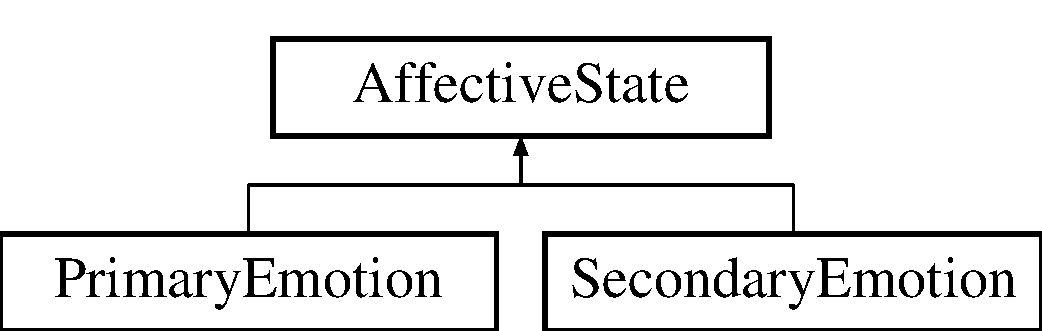
\includegraphics[height=2.000000cm]{class_affective_state}
\end{center}
\end{figure}
\subsection*{\-Public \-Types}
\begin{DoxyCompactItemize}
\item 
enum \hyperlink{class_affective_state_aa47963a65353591a1e2109987ef624a1}{decay\-Function\-Enum} \{ {\bfseries \-N\-O\-N\-E} =  0, 
{\bfseries \-L\-I\-N\-E\-A\-R} =  1, 
{\bfseries \-E\-X\-P\-O\-N\-E\-N\-T\-I\-A\-L} =  2, 
{\bfseries \-C\-O\-S\-I\-N\-E} =  3
 \}
\end{DoxyCompactItemize}
\subsection*{\-Public \-Member \-Functions}
\begin{DoxyCompactItemize}
\item 
\hypertarget{class_affective_state_a65e6807f1091c79f44a84c95adb1b4fd}{
\hyperlink{class_affective_state_a65e6807f1091c79f44a84c95adb1b4fd}{\-Affective\-State} ()}
\label{class_affective_state_a65e6807f1091c79f44a84c95adb1b4fd}

\begin{DoxyCompactList}\small\item\em \-Default \-Constructor. \end{DoxyCompactList}\item 
\hypertarget{class_affective_state_a8573788f95c382b5eb6037a2b4f3aa1a}{
\hyperlink{class_affective_state_a8573788f95c382b5eb6037a2b4f3aa1a}{\-Affective\-State} (const \hyperlink{class_affective_state}{\-Affective\-State} \&as)}
\label{class_affective_state_a8573788f95c382b5eb6037a2b4f3aa1a}

\begin{DoxyCompactList}\small\item\em \-Copy \-Constructor. \end{DoxyCompactList}\item 
\hypertarget{class_affective_state_af9b8433c91ed8e02978c3b42ed5ac6b4}{
{\bfseries \-Affective\-State} (std\-::vector$<$ \hyperlink{class_affect_polygon}{\-Affect\-Polygon} $\ast$ $>$ ap\-\_\-vec)}
\label{class_affective_state_af9b8433c91ed8e02978c3b42ed5ac6b4}

\item 
\hypertarget{class_affective_state_a08fc349147b79539acd264b73cec7f26}{
{\bfseries \-Affective\-State} (\hyperlink{class_affect_polygon}{\-Affect\-Polygon} $\ast$ap)}
\label{class_affective_state_a08fc349147b79539acd264b73cec7f26}

\item 
bool \hyperlink{class_affective_state_af7ac4f21de22c0ab43e3889458c61ff2}{add\-Polygon} (std\-::vector$<$ \hyperlink{class_affect_polygon}{\-Affect\-Polygon} $\ast$ $>$ data)
\item 
\hypertarget{class_affective_state_a0736c2a1ef6341a6220e10460eeda7dc}{
bool {\bfseries add\-Polygon} (\hyperlink{class_affect_polygon}{\-Affect\-Polygon} $\ast$polygon)}
\label{class_affective_state_a0736c2a1ef6341a6220e10460eeda7dc}

\item 
bool \hyperlink{class_affective_state_a3b824330921fc05fe7dd2f49eec150d2}{set\-Lifetime} (double new\-Lifetime)
\item 
bool \hyperlink{class_affective_state_ae03bf91dc1939016fcd45ceb60e7cbf5}{set\-Lifetime} ()
\item 
\hypertarget{class_affective_state_a7054661d256830354e34c71549d2b4ae}{
bool \hyperlink{class_affective_state_a7054661d256830354e34c71549d2b4ae}{trigger} (double \-\_\-lifetime=-\/1)}
\label{class_affective_state_a7054661d256830354e34c71549d2b4ae}

\begin{DoxyCompactList}\small\item\em to make it easier to \char`\"{}trigger\char`\"{} an \hyperlink{class_affective_state}{\-Affective\-State} \end{DoxyCompactList}\item 
\hypertarget{class_affective_state_a42be8cbd6088728f2d4995c405373204}{
bool {\bfseries set\-Standard\-Lifetime} (double new\-Lifetime)}
\label{class_affective_state_a42be8cbd6088728f2d4995c405373204}

\item 
\hypertarget{class_affective_state_aac1d520a62c463f763060144ea2907b9}{
bool {\bfseries set\-Base\-Intensity} (double new\-Intensity)}
\label{class_affective_state_aac1d520a62c463f763060144ea2907b9}

\item 
\hypertarget{class_affective_state_a26df2365c23db0ecf640a06075a224b0}{
double {\bfseries get\-Lifetime} ()}
\label{class_affective_state_a26df2365c23db0ecf640a06075a224b0}

\item 
void \hyperlink{class_affective_state_ad0208fab4ea9bf577155c8aae932c96b}{set\-Decay\-Function} (\hyperlink{class_affective_state_aa47963a65353591a1e2109987ef624a1}{decay\-Function\-Enum} decay\-Func, double decay\-Param=0.\-0)
\item 
\hypertarget{class_affective_state_a9e2e8399228a86af59cdb7406aae9813}{
int {\bfseries get\-Decay\-Function} ()}
\label{class_affective_state_a9e2e8399228a86af59cdb7406aae9813}

\item 
std\-::vector$<$ \hyperlink{class_affect_vertex}{\-Affect\-Vertex} $\ast$ $>$ \hyperlink{class_affective_state_a3e447cea61d9d9dc7b758a68a4e8e009}{get\-Likelihood} ()
\item 
\hypertarget{class_affective_state_a4093ad8a30493c8f35d400b869a33968}{
void \hyperlink{class_affective_state_a4093ad8a30493c8f35d400b869a33968}{set\-I\-D} (int idnew)}
\label{class_affective_state_a4093ad8a30493c8f35d400b869a33968}

\begin{DoxyCompactList}\small\item\em getter und setter for the \-I\-D \end{DoxyCompactList}\item 
\hypertarget{class_affective_state_a22f046f76fb1c1176ec49b803da09b8f}{
int {\bfseries get\-I\-D} () const }
\label{class_affective_state_a22f046f76fb1c1176ec49b803da09b8f}

\item 
\hypertarget{class_affective_state_ab37b59269cf599a28e0cb2f8aa083e38}{
const double {\bfseries get\-Intensity} () const }
\label{class_affective_state_ab37b59269cf599a28e0cb2f8aa083e38}

\item 
\hypertarget{class_affective_state_a82b0f96a1494f5c58a6bec2840f3728a}{
void \hyperlink{class_affective_state_a82b0f96a1494f5c58a6bec2840f3728a}{update} (float dt)}
\label{class_affective_state_a82b0f96a1494f5c58a6bec2840f3728a}

\begin{DoxyCompactList}\small\item\em \-Will update the intensity value according to the decay function und relative to the dt. \end{DoxyCompactList}\item 
void \hyperlink{class_affective_state_a0c6f905934f6abe08a64d3b25fe88ff1}{set\-Emotion\-Container} (\hyperlink{class_emotion_dynamics}{\-Emotion\-Dynamics} $\ast$new\-Emo\-Con)
\item 
bool \hyperlink{class_affective_state_a913bce75bbf5bb870207e69fefb5efef}{set\-Likelihood} (float new\-Likelihood)
\item 
\hypertarget{class_affective_state_abe11a841bcd9979d183a946b476142d8}{
void \hyperlink{class_affective_state_abe11a841bcd9979d183a946b476142d8}{dump} (std\-::ostream \&)}
\label{class_affective_state_abe11a841bcd9979d183a946b476142d8}

\begin{DoxyCompactList}\small\item\em \-Dump to stream for debugging. \end{DoxyCompactList}\item 
void \hyperlink{class_affective_state_add666df993512c3af62ad1b6b00cab18}{update\-Likelihood} ()
\end{DoxyCompactItemize}
\subsection*{\-Public \-Attributes}
\begin{DoxyCompactItemize}
\item 
std\-::string \hyperlink{class_affective_state_ad46f24a9835b890cfe147ae0463d01bf}{type}
\item 
std\-::vector$<$ std\-::string $>$ \hyperlink{class_affective_state_a80a1bb184121a40c28c1d3ff103fd47f}{tokens}
\item 
\hypertarget{class_affective_state_a755c41239bc7777bfcc962a12768b27e}{
\hyperlink{class_emotion_dynamics}{\-Emotion\-Dynamics} $\ast$ {\bfseries emo\-Con}}
\label{class_affective_state_a755c41239bc7777bfcc962a12768b27e}

\item 
std\-::vector$<$ \hyperlink{class_affect_polygon}{\-Affect\-Polygon} $\ast$ $>$ \hyperlink{class_affective_state_ac2ea3391ebe5fd5708aecb2acdb7fe0d}{polygons}
\end{DoxyCompactItemize}
\subsection*{\-Protected \-Member \-Functions}
\begin{DoxyCompactItemize}
\item 
std\-::vector$<$ \hyperlink{class_affect_vertex}{\-Affect\-Vertex} $\ast$ $>$ \hyperlink{class_affective_state_a6529b00f1d62e79c8db2d09d756f011a}{update\-Likelihood} (std\-::vector$<$ int $>$ \-P\-A\-D)
\item 
bool \hyperlink{class_affective_state_a952cec059138bd392c5897a18ed3b6cd}{set\-Intensity} (double new\-Intensity)
\end{DoxyCompactItemize}
\subsection*{\-Protected \-Attributes}
\begin{DoxyCompactItemize}
\item 
double \hyperlink{class_affective_state_ae067f508a2053daf7541bf0901e38b67}{lifetime}
\item 
double \hyperlink{class_affective_state_a081f3fff485d06a746b1b472adf3160c}{standard\-Lifetime}
\item 
double \hyperlink{class_affective_state_a3ab3863056c40d2bd2910642d5565dc6}{base\-Intensity}
\item 
int \hyperlink{class_affective_state_a5db5a1c7f76aba385d216010bcc74509}{id}
\item 
\hypertarget{class_affective_state_a670e6974b030651725a83b379f233711}{
\hyperlink{class_affective_state_aa47963a65353591a1e2109987ef624a1}{decay\-Function\-Enum} {\bfseries decay\-Function}}
\label{class_affective_state_a670e6974b030651725a83b379f233711}

\item 
double \hyperlink{class_affective_state_a80ee188d27e7b36c94ac9c1f9ddb3cb7}{decay\-Parameter}
\item 
std\-::vector$<$ \hyperlink{class_affect_vertex}{\-Affect\-Vertex} $\ast$ $>$ \hyperlink{class_affective_state_a7dedd88cae5c125dfedaaf2eb48ae01f}{likelihoods}
\end{DoxyCompactItemize}


\subsection{\-Detailed \-Description}
\-An \hyperlink{class_affective_state}{\-Affective\-State} is the base class of all \-Primary and \-Secondary emotions. 

\-Definition at line 129 of file \-Affective\-State.\-h.



\subsection{\-Member \-Enumeration \-Documentation}
\hypertarget{class_affective_state_aa47963a65353591a1e2109987ef624a1}{
\index{\-Affective\-State@{\-Affective\-State}!decay\-Function\-Enum@{decay\-Function\-Enum}}
\index{decay\-Function\-Enum@{decay\-Function\-Enum}!AffectiveState@{\-Affective\-State}}
\subsubsection[{decay\-Function\-Enum}]{\setlength{\rightskip}{0pt plus 5cm}enum {\bf \-Affective\-State\-::decay\-Function\-Enum}}}
\label{class_affective_state_aa47963a65353591a1e2109987ef624a1}
\-The following enumeration denotes the possible decay functions. \-D\-E\-F\-A\-U\-L\-T\-: \-N\-O\-N\-E 

\-Definition at line 173 of file \-Affective\-State.\-h.



\subsection{\-Member \-Function \-Documentation}
\hypertarget{class_affective_state_af7ac4f21de22c0ab43e3889458c61ff2}{
\index{\-Affective\-State@{\-Affective\-State}!add\-Polygon@{add\-Polygon}}
\index{add\-Polygon@{add\-Polygon}!AffectiveState@{\-Affective\-State}}
\subsubsection[{add\-Polygon}]{\setlength{\rightskip}{0pt plus 5cm}bool \-Affective\-State\-::add\-Polygon (
\begin{DoxyParamCaption}
\item[{std\-::vector$<$ {\bf \-Affect\-Polygon} $\ast$ $>$}]{data}
\end{DoxyParamCaption}
)}}
\label{class_affective_state_af7ac4f21de22c0ab43e3889458c61ff2}
\-Will be used to add a point, i.\-e. a polygon with only one vertex, a line, i.\-e. a polygon with only two vertices, or a polygon with (more than two) vertices lying all in the same plane (+/-\/ 100 \-D) to the existing \-P\-A\-D\-Values. 

\-Definition at line 266 of file \-Affective\-State.\-cc.

\hypertarget{class_affective_state_a3e447cea61d9d9dc7b758a68a4e8e009}{
\index{\-Affective\-State@{\-Affective\-State}!get\-Likelihood@{get\-Likelihood}}
\index{get\-Likelihood@{get\-Likelihood}!AffectiveState@{\-Affective\-State}}
\subsubsection[{get\-Likelihood}]{\setlength{\rightskip}{0pt plus 5cm}vector$<$ {\bf \-Affect\-Vertex} $\ast$ $>$ \-Affective\-State\-::get\-Likelihood (
\begin{DoxyParamCaption}
{}
\end{DoxyParamCaption}
)}}
\label{class_affective_state_a3e447cea61d9d9dc7b758a68a4e8e009}
\-Without an argument given we try to use the \hyperlink{class_emotion_container}{\-Emotion\-Container} emo\-Con to get the \-P\-A\-D values of the \-Emotional\-Attendee.

\-Calculate the likelihood of this \hyperlink{class_affective_state}{\-Affective\-State} with respect to the data in the \hyperlink{class_emotion_container}{\-Emotion\-Container} emo\-Con, if it is set. 

\-Definition at line 184 of file \-Affective\-State.\-cc.

\hypertarget{class_affective_state_ad0208fab4ea9bf577155c8aae932c96b}{
\index{\-Affective\-State@{\-Affective\-State}!set\-Decay\-Function@{set\-Decay\-Function}}
\index{set\-Decay\-Function@{set\-Decay\-Function}!AffectiveState@{\-Affective\-State}}
\subsubsection[{set\-Decay\-Function}]{\setlength{\rightskip}{0pt plus 5cm}void \-Affective\-State\-::set\-Decay\-Function (
\begin{DoxyParamCaption}
\item[{{\bf decay\-Function\-Enum}}]{decay\-Func, }
\item[{double}]{decay\-Param = {\ttfamily 0.0}}
\end{DoxyParamCaption}
)}}
\label{class_affective_state_ad0208fab4ea9bf577155c8aae932c96b}
\-To set a new decay function for the current emotion. \-We won't reset the intesity value here. 

\-Definition at line 151 of file \-Affective\-State.\-cc.

\hypertarget{class_affective_state_a0c6f905934f6abe08a64d3b25fe88ff1}{
\index{\-Affective\-State@{\-Affective\-State}!set\-Emotion\-Container@{set\-Emotion\-Container}}
\index{set\-Emotion\-Container@{set\-Emotion\-Container}!AffectiveState@{\-Affective\-State}}
\subsubsection[{set\-Emotion\-Container}]{\setlength{\rightskip}{0pt plus 5cm}void \-Affective\-State\-::set\-Emotion\-Container (
\begin{DoxyParamCaption}
\item[{{\bf \-Emotion\-Dynamics} $\ast$}]{new\-Emo\-Con}
\end{DoxyParamCaption}
)\hspace{0.3cm}{\ttfamily  \mbox{[}inline\mbox{]}}}}
\label{class_affective_state_a0c6f905934f6abe08a64d3b25fe88ff1}
\-Now we want to be able to set a reference to an emotion container emo\-Con such that we can easily use the \-Emotion\-Container's variables. 

\-Definition at line 214 of file \-Affective\-State.\-h.

\hypertarget{class_affective_state_a952cec059138bd392c5897a18ed3b6cd}{
\index{\-Affective\-State@{\-Affective\-State}!set\-Intensity@{set\-Intensity}}
\index{set\-Intensity@{set\-Intensity}!AffectiveState@{\-Affective\-State}}
\subsubsection[{set\-Intensity}]{\setlength{\rightskip}{0pt plus 5cm}bool \-Affective\-State\-::set\-Intensity (
\begin{DoxyParamCaption}
\item[{double}]{new\-Intensity}
\end{DoxyParamCaption}
)\hspace{0.3cm}{\ttfamily  \mbox{[}protected\mbox{]}}}}
\label{class_affective_state_a952cec059138bd392c5897a18ed3b6cd}
\-To set the intensity if it lies within \mbox{[}0.\-0, 1.\-0\mbox{]} returns success or failure 

\-Definition at line 339 of file \-Affective\-State.\-cc.

\hypertarget{class_affective_state_a3b824330921fc05fe7dd2f49eec150d2}{
\index{\-Affective\-State@{\-Affective\-State}!set\-Lifetime@{set\-Lifetime}}
\index{set\-Lifetime@{set\-Lifetime}!AffectiveState@{\-Affective\-State}}
\subsubsection[{set\-Lifetime}]{\setlength{\rightskip}{0pt plus 5cm}bool \-Affective\-State\-::set\-Lifetime (
\begin{DoxyParamCaption}
\item[{double}]{new\-Lifetime}
\end{DoxyParamCaption}
)}}
\label{class_affective_state_a3b824330921fc05fe7dd2f49eec150d2}
\-This will set the new lifetime in seconds. \-We recalculate the decay\-Parameter to ensure the correct lifetime with respect to the dt value of the \hyperlink{class_emotion_container}{\-Emotion\-Container} emo\-Con-\/$>$dt. \-We will also reset the intensity value to 1.\-0! 

\-Definition at line 105 of file \-Affective\-State.\-cc.

\hypertarget{class_affective_state_ae03bf91dc1939016fcd45ceb60e7cbf5}{
\index{\-Affective\-State@{\-Affective\-State}!set\-Lifetime@{set\-Lifetime}}
\index{set\-Lifetime@{set\-Lifetime}!AffectiveState@{\-Affective\-State}}
\subsubsection[{set\-Lifetime}]{\setlength{\rightskip}{0pt plus 5cm}bool \-Affective\-State\-::set\-Lifetime (
\begin{DoxyParamCaption}
{}
\end{DoxyParamCaption}
)\hspace{0.3cm}{\ttfamily  \mbox{[}inline\mbox{]}}}}
\label{class_affective_state_ae03bf91dc1939016fcd45ceb60e7cbf5}
\-For convenience we can call this function without parameter. \-The standard lifetime will be set. 

\-Definition at line 159 of file \-Affective\-State.\-h.

\hypertarget{class_affective_state_a913bce75bbf5bb870207e69fefb5efef}{
\index{\-Affective\-State@{\-Affective\-State}!set\-Likelihood@{set\-Likelihood}}
\index{set\-Likelihood@{set\-Likelihood}!AffectiveState@{\-Affective\-State}}
\subsubsection[{set\-Likelihood}]{\setlength{\rightskip}{0pt plus 5cm}bool \-Affective\-State\-::set\-Likelihood (
\begin{DoxyParamCaption}
\item[{float}]{new\-Likelihood}
\end{DoxyParamCaption}
)}}
\label{class_affective_state_a913bce75bbf5bb870207e69fefb5efef}
\-In case our \hyperlink{class_emotion_container}{\-Emotion\-Container} is set to \char`\"{}is\-Active == false\char`\"{} we might call this function to \-M\-A\-N\-U\-A\-L\-L\-Y set the likelihood. 

\-Definition at line 377 of file \-Affective\-State.\-cc.

\hypertarget{class_affective_state_add666df993512c3af62ad1b6b00cab18}{
\index{\-Affective\-State@{\-Affective\-State}!update\-Likelihood@{update\-Likelihood}}
\index{update\-Likelihood@{update\-Likelihood}!AffectiveState@{\-Affective\-State}}
\subsubsection[{update\-Likelihood}]{\setlength{\rightskip}{0pt plus 5cm}void \-Affective\-State\-::update\-Likelihood (
\begin{DoxyParamCaption}
{}
\end{DoxyParamCaption}
)}}
\label{class_affective_state_add666df993512c3af62ad1b6b00cab18}
updating all likelihoods of this affective state. \-Should be called within \hyperlink{class_affective_state_a82b0f96a1494f5c58a6bec2840f3728a}{update(float dt)}.

\-Calculate the likelihood of this \hyperlink{class_affective_state}{\-Affective\-State} with respect to the data in the \hyperlink{class_emotion_container}{\-Emotion\-Container} emo\-Con, if it is set. 

\-Definition at line 166 of file \-Affective\-State.\-cc.

\hypertarget{class_affective_state_a6529b00f1d62e79c8db2d09d756f011a}{
\index{\-Affective\-State@{\-Affective\-State}!update\-Likelihood@{update\-Likelihood}}
\index{update\-Likelihood@{update\-Likelihood}!AffectiveState@{\-Affective\-State}}
\subsubsection[{update\-Likelihood}]{\setlength{\rightskip}{0pt plus 5cm}std\-::vector$<${\bf \-Affect\-Vertex}$\ast$$>$ \-Affective\-State\-::update\-Likelihood (
\begin{DoxyParamCaption}
\item[{std\-::vector$<$ int $>$}]{\-P\-A\-D}
\end{DoxyParamCaption}
)\hspace{0.3cm}{\ttfamily  \mbox{[}protected\mbox{]}}}}
\label{class_affective_state_a6529b00f1d62e79c8db2d09d756f011a}
\-Will return the likelihood of the affective state to become aware. \-All the magic is to be done here\-: 1. \-We will calculate the distance between \-P\-A\-D and affective state's \-Polygons. 2. \-We take into account min/max\-\_\-distances to calculate activation. 3. likelihood(t) = activation(t) $\ast$ intensity(t) \-If we have several polygons in the vector, we have to take the best match in step 1, i.\-e. the one with the closest distance. \-If the affective state is represented as a polygon, we take the minimum distance to the \-P\-O\-L\-Y\-G\-O\-N instead of the \-P\-O\-I\-N\-T\-S. 

\subsection{\-Member \-Data \-Documentation}
\hypertarget{class_affective_state_a3ab3863056c40d2bd2910642d5565dc6}{
\index{\-Affective\-State@{\-Affective\-State}!base\-Intensity@{base\-Intensity}}
\index{base\-Intensity@{base\-Intensity}!AffectiveState@{\-Affective\-State}}
\subsubsection[{base\-Intensity}]{\setlength{\rightskip}{0pt plus 5cm}double {\bf \-Affective\-State\-::base\-Intensity}\hspace{0.3cm}{\ttfamily  \mbox{[}protected\mbox{]}}}}
\label{class_affective_state_a3ab3863056c40d2bd2910642d5565dc6}
\-This can be set at the beginning and will be used when lifetime == -\/1 \-D\-E\-F\-A\-U\-L\-T\-: 1.\-0 

\-Definition at line 267 of file \-Affective\-State.\-h.

\hypertarget{class_affective_state_a80ee188d27e7b36c94ac9c1f9ddb3cb7}{
\index{\-Affective\-State@{\-Affective\-State}!decay\-Parameter@{decay\-Parameter}}
\index{decay\-Parameter@{decay\-Parameter}!AffectiveState@{\-Affective\-State}}
\subsubsection[{decay\-Parameter}]{\setlength{\rightskip}{0pt plus 5cm}double {\bf \-Affective\-State\-::decay\-Parameter}\hspace{0.3cm}{\ttfamily  \mbox{[}protected\mbox{]}}}}
\label{class_affective_state_a80ee188d27e7b36c94ac9c1f9ddb3cb7}
\-A possible parameter for the decay functions. \-D\-E\-F\-A\-U\-L\-T\-: 1.\-0 

\-Definition at line 279 of file \-Affective\-State.\-h.

\hypertarget{class_affective_state_a5db5a1c7f76aba385d216010bcc74509}{
\index{\-Affective\-State@{\-Affective\-State}!id@{id}}
\index{id@{id}!AffectiveState@{\-Affective\-State}}
\subsubsection[{id}]{\setlength{\rightskip}{0pt plus 5cm}int {\bf \-Affective\-State\-::id}\hspace{0.3cm}{\ttfamily  \mbox{[}protected\mbox{]}}}}
\label{class_affective_state_a5db5a1c7f76aba385d216010bcc74509}
\-For backward compatibility we include an id being one of the \char`\"{}\-M\-O\-O\-D\-S\char`\"{} defined above \-D\-E\-F\-A\-U\-L\-T\-: \-M\-O\-O\-D\-\_\-\-N\-E\-U\-T\-R\-A\-L. 

\-Definition at line 272 of file \-Affective\-State.\-h.

\hypertarget{class_affective_state_ae067f508a2053daf7541bf0901e38b67}{
\index{\-Affective\-State@{\-Affective\-State}!lifetime@{lifetime}}
\index{lifetime@{lifetime}!AffectiveState@{\-Affective\-State}}
\subsubsection[{lifetime}]{\setlength{\rightskip}{0pt plus 5cm}double {\bf \-Affective\-State\-::lifetime}\hspace{0.3cm}{\ttfamily  \mbox{[}protected\mbox{]}}}}
\label{class_affective_state_ae067f508a2053daf7541bf0901e38b67}
\-Every affective state (primary or secondary) may have a \char`\"{}lifetime\char`\"{} now. \-Together with the decay function below, we can realize a context dependent turning on/off of esp. secondary emotions. \-A lifetime of \char`\"{}-\/1.\-0\char`\"{} is interpreted as \char`\"{}always on\char`\"{} and should be the \-D\-E\-F\-A\-U\-L\-T value. 

\-Definition at line 257 of file \-Affective\-State.\-h.

\hypertarget{class_affective_state_a7dedd88cae5c125dfedaaf2eb48ae01f}{
\index{\-Affective\-State@{\-Affective\-State}!likelihoods@{likelihoods}}
\index{likelihoods@{likelihoods}!AffectiveState@{\-Affective\-State}}
\subsubsection[{likelihoods}]{\setlength{\rightskip}{0pt plus 5cm}std\-::vector$<${\bf \-Affect\-Vertex}$\ast$$>$ {\bf \-Affective\-State\-::likelihoods}\hspace{0.3cm}{\ttfamily  \mbox{[}protected\mbox{]}}}}
\label{class_affective_state_a7dedd88cae5c125dfedaaf2eb48ae01f}
\-Keeping track of the \-Affective\-State's likelihood. \-Updated automatically within \hyperlink{class_affective_state_a82b0f96a1494f5c58a6bec2840f3728a}{update(float dt)}. 

\-Definition at line 290 of file \-Affective\-State.\-h.

\hypertarget{class_affective_state_ac2ea3391ebe5fd5708aecb2acdb7fe0d}{
\index{\-Affective\-State@{\-Affective\-State}!polygons@{polygons}}
\index{polygons@{polygons}!AffectiveState@{\-Affective\-State}}
\subsubsection[{polygons}]{\setlength{\rightskip}{0pt plus 5cm}std\-::vector$<${\bf \-Affect\-Polygon}$\ast$$>$ {\bf \-Affective\-State\-::polygons}}}
\label{class_affective_state_ac2ea3391ebe5fd5708aecb2acdb7fe0d}
\-Vector of \-Affect\-Polygons \-Every primary as well as secondary emotion is to be represented in \-P\-A\-D \-Space \-D\-E\-F\-A\-U\-L\-T\-: empty vector. 

\-Definition at line 221 of file \-Affective\-State.\-h.

\hypertarget{class_affective_state_a081f3fff485d06a746b1b472adf3160c}{
\index{\-Affective\-State@{\-Affective\-State}!standard\-Lifetime@{standard\-Lifetime}}
\index{standard\-Lifetime@{standard\-Lifetime}!AffectiveState@{\-Affective\-State}}
\subsubsection[{standard\-Lifetime}]{\setlength{\rightskip}{0pt plus 5cm}double {\bf \-Affective\-State\-::standard\-Lifetime}\hspace{0.3cm}{\ttfamily  \mbox{[}protected\mbox{]}}}}
\label{class_affective_state_a081f3fff485d06a746b1b472adf3160c}
\-We might set a standard lifetime for every \-A\-S \-D\-E\-F\-A\-U\-L\-T\-: -\/1.\-0, i.\-e. always on 

\-Definition at line 262 of file \-Affective\-State.\-h.

\hypertarget{class_affective_state_a80a1bb184121a40c28c1d3ff103fd47f}{
\index{\-Affective\-State@{\-Affective\-State}!tokens@{tokens}}
\index{tokens@{tokens}!AffectiveState@{\-Affective\-State}}
\subsubsection[{tokens}]{\setlength{\rightskip}{0pt plus 5cm}std\-::vector$<$std\-::string$>$ {\bf \-Affective\-State\-::tokens}}}
\label{class_affective_state_a80a1bb184121a40c28c1d3ff103fd47f}
\-This might be a list of tokens \-D\-E\-F\-A\-U\-L\-T\-: empty 

\-Definition at line 209 of file \-Affective\-State.\-h.

\hypertarget{class_affective_state_ad46f24a9835b890cfe147ae0463d01bf}{
\index{\-Affective\-State@{\-Affective\-State}!type@{type}}
\index{type@{type}!AffectiveState@{\-Affective\-State}}
\subsubsection[{type}]{\setlength{\rightskip}{0pt plus 5cm}std\-::string {\bf \-Affective\-State\-::type}}}
\label{class_affective_state_ad46f24a9835b890cfe147ae0463d01bf}
\-This will be the \-O\-C\-C / \-Scherer / \-Becker string denoting the type or class of emotion \-D\-E\-F\-A\-U\-L\-T\-: undefined 

\-Definition at line 204 of file \-Affective\-State.\-h.



\-The documentation for this class was generated from the following files\-:\begin{DoxyCompactItemize}
\item 
\-Affective\-State.\-h\item 
\-Affective\-State.\-cc\end{DoxyCompactItemize}

\hypertarget{class_affect_polygon}{
\section{\-Affect\-Polygon \-Class \-Reference}
\label{class_affect_polygon}\index{\-Affect\-Polygon@{\-Affect\-Polygon}}
}


{\ttfamily \#include $<$\-Affective\-State.\-h$>$}

\subsection*{\-Public \-Member \-Functions}
\begin{DoxyCompactItemize}
\item 
\hypertarget{class_affect_polygon_a364e906c60057bc9a6264221ba52b1bf}{
{\bfseries \-Affect\-Polygon} (std\-::vector$<$ \hyperlink{class_affect_vertex}{\-Affect\-Vertex} $\ast$ $>$, std\-::string \hyperlink{class_affect_polygon_aea731a4d326a3095686b529030266188}{gl\-Mode}=\char`\"{}\-G\-L\-\_\-\-P\-O\-I\-N\-T\-S\char`\"{})}
\label{class_affect_polygon_a364e906c60057bc9a6264221ba52b1bf}

\item 
\hypertarget{class_affect_polygon_adee033730c99195b8c6261a9530f86b4}{
{\bfseries \-Affect\-Polygon} (\hyperlink{class_affect_vertex}{\-Affect\-Vertex} $\ast$)}
\label{class_affect_polygon_adee033730c99195b8c6261a9530f86b4}

\item 
bool \hyperlink{class_affect_polygon_a8483a6d1e2f22bd6d975aad7521c3761}{valid} ()
\item 
\hypertarget{class_affect_polygon_a7af2c3c08a837bff793e6be83c81b81c}{
void \hyperlink{class_affect_polygon_a7af2c3c08a837bff793e6be83c81b81c}{add\-Vertices} (std\-::vector$<$ \hyperlink{class_affect_vertex}{\-Affect\-Vertex} $\ast$ $>$)}
\label{class_affect_polygon_a7af2c3c08a837bff793e6be83c81b81c}

\begin{DoxyCompactList}\small\item\em \-To add vertices to the polygon. \end{DoxyCompactList}\item 
\hypertarget{class_affect_polygon_a034a7b375339e53b42ebf25d94c0a76c}{
float {\bfseries get\-Intensity} (int p, int a, int d)}
\label{class_affect_polygon_a034a7b375339e53b42ebf25d94c0a76c}

\item 
\hypertarget{class_affect_polygon_a6ee97313e0d1f4199e275579142d8ea5}{
std\-::vector$<$ float $>$ {\bfseries linear\-Interpolation} (\hyperlink{class_affect_vertex}{\-Affect\-Vertex} const \&v1, \hyperlink{class_affect_vertex}{\-Affect\-Vertex} const \&v2, int coord\mbox{[}$\,$\mbox{]})}
\label{class_affect_polygon_a6ee97313e0d1f4199e275579142d8ea5}

\end{DoxyCompactItemize}
\subsection*{\-Public \-Attributes}
\begin{DoxyCompactItemize}
\item 
\hypertarget{class_affect_polygon_a9184c5ecb96030b1b20d9f1b856f3c40}{
std\-::vector$<$ \hyperlink{class_affect_vertex}{\-Affect\-Vertex} $\ast$ $>$ {\bfseries vertices}}
\label{class_affect_polygon_a9184c5ecb96030b1b20d9f1b856f3c40}

\item 
float \hyperlink{class_affect_polygon_abc171095a4d763dbf133ac8d3c5faa27}{min\-\_\-distance}
\item 
\hypertarget{class_affect_polygon_a2f4af25cbbb2d4ab36fe3d3dd71b678b}{
float {\bfseries max\-\_\-distance}}
\label{class_affect_polygon_a2f4af25cbbb2d4ab36fe3d3dd71b678b}

\item 
std\-::string \hyperlink{class_affect_polygon_aea731a4d326a3095686b529030266188}{gl\-Mode}
\end{DoxyCompactItemize}


\subsection{\-Detailed \-Description}
\hyperlink{class_affect_polygon}{\-Affect\-Polygon} used for representation of an \hyperlink{class_affective_state}{\-Affective\-State} in \-P\-A\-D-\/space. \-Uses \-Affect\-Vertices as described above. 

\-Definition at line 85 of file \-Affective\-State.\-h.



\subsection{\-Member \-Function \-Documentation}
\hypertarget{class_affect_polygon_a8483a6d1e2f22bd6d975aad7521c3761}{
\index{\-Affect\-Polygon@{\-Affect\-Polygon}!valid@{valid}}
\index{valid@{valid}!AffectPolygon@{\-Affect\-Polygon}}
\subsubsection[{valid}]{\setlength{\rightskip}{0pt plus 5cm}bool \-Affect\-Polygon\-::valid (
\begin{DoxyParamCaption}
{}
\end{DoxyParamCaption}
)}}
\label{class_affect_polygon_a8483a6d1e2f22bd6d975aad7521c3761}
\-Tests the polygon for validity, i.\-e. if all \-D-\/values lie in the same plane. 

\-Definition at line 496 of file \-Affective\-State.\-cc.



\subsection{\-Member \-Data \-Documentation}
\hypertarget{class_affect_polygon_aea731a4d326a3095686b529030266188}{
\index{\-Affect\-Polygon@{\-Affect\-Polygon}!gl\-Mode@{gl\-Mode}}
\index{gl\-Mode@{gl\-Mode}!AffectPolygon@{\-Affect\-Polygon}}
\subsubsection[{gl\-Mode}]{\setlength{\rightskip}{0pt plus 5cm}std\-::string {\bf \-Affect\-Polygon\-::gl\-Mode}}}
\label{class_affect_polygon_aea731a4d326a3095686b529030266188}
get the \-G\-L\-\_\-\-M\-O\-D\-E \-D\-E\-F\-A\-U\-L\-T\-: \-G\-L\-\_\-\-P\-O\-I\-N\-T 

\-Definition at line 115 of file \-Affective\-State.\-h.

\hypertarget{class_affect_polygon_abc171095a4d763dbf133ac8d3c5faa27}{
\index{\-Affect\-Polygon@{\-Affect\-Polygon}!min\-\_\-distance@{min\-\_\-distance}}
\index{min\-\_\-distance@{min\-\_\-distance}!AffectPolygon@{\-Affect\-Polygon}}
\subsubsection[{min\-\_\-distance}]{\setlength{\rightskip}{0pt plus 5cm}float {\bf \-Affect\-Polygon\-::min\-\_\-distance}}}
\label{class_affect_polygon_abc171095a4d763dbf133ac8d3c5faa27}
min\-\_\-distance and max\-\_\-distance are now substituting the activation and saturation thresholds of the original implementation of 2003 \-D\-E\-F\-A\-L\-U\-T\-S\-: min\-\_\-distance = outer\-Radius = 0.\-64, max\-\_\-distance = inner\-Radius = 0.\-2 

\-Definition at line 108 of file \-Affective\-State.\-h.



\-The documentation for this class was generated from the following files\-:\begin{DoxyCompactItemize}
\item 
\-Affective\-State.\-h\item 
\-Affective\-State.\-cc\end{DoxyCompactItemize}

\hypertarget{class_affect_vertex}{
\section{\-Affect\-Vertex \-Class \-Reference}
\label{class_affect_vertex}\index{\-Affect\-Vertex@{\-Affect\-Vertex}}
}


{\ttfamily \#include $<$\-Affective\-State.\-h$>$}

\subsection*{\-Public \-Member \-Functions}
\begin{DoxyCompactItemize}
\item 
\hypertarget{class_affect_vertex_a50e338d93dd0a38d4089fc14284761a4}{
{\bfseries \-Affect\-Vertex} (int data\mbox{[}3\mbox{]})}
\label{class_affect_vertex_a50e338d93dd0a38d4089fc14284761a4}

\item 
\hypertarget{class_affect_vertex_aec1f32cfd8c8fa579a1adbbc34af4d24}{
{\bfseries \-Affect\-Vertex} (int data\mbox{[}3\mbox{]}, double intens)}
\label{class_affect_vertex_aec1f32cfd8c8fa579a1adbbc34af4d24}

\item 
\hypertarget{class_affect_vertex_a6ca4a6bf072257b5accc4389f3f6e6e5}{
bool {\bfseries valid} ()}
\label{class_affect_vertex_a6ca4a6bf072257b5accc4389f3f6e6e5}

\end{DoxyCompactItemize}
\subsection*{\-Public \-Attributes}
\begin{DoxyCompactItemize}
\item 
\hypertarget{class_affect_vertex_a0ffa48aa0df4356da53708a938e53e83}{
int {\bfseries coords} \mbox{[}3\mbox{]}}
\label{class_affect_vertex_a0ffa48aa0df4356da53708a938e53e83}

\item 
\hypertarget{class_affect_vertex_a9742362a1036509af353b1fa7d5d382b}{
float {\bfseries intensity}}
\label{class_affect_vertex_a9742362a1036509af353b1fa7d5d382b}

\item 
\hypertarget{class_affect_vertex_aa659889f294516bbb779909dbf83a1ed}{
float {\bfseries likelihood}}
\label{class_affect_vertex_aa659889f294516bbb779909dbf83a1ed}

\end{DoxyCompactItemize}


\subsection{\-Detailed \-Description}
\hyperlink{class_affect_vertex}{\-Affect\-Vertex} used for representation of an \hyperlink{class_affective_state}{\-Affective\-State} in \-P\-A\-D-\/space. \-If we want to biuld a polygon, we might use several of these together with intensity values to acquire a \char`\"{}region in P\-A\-D-\/space\char`\"{}. 

\-Definition at line 60 of file \-Affective\-State.\-h.



\-The documentation for this class was generated from the following files\-:\begin{DoxyCompactItemize}
\item 
\-Affective\-State.\-h\item 
\-Affective\-State.\-cc\end{DoxyCompactItemize}

\hypertarget{classcoga_attendee}{
\section{coga\-Attendee \-Class \-Reference}
\label{classcoga_attendee}\index{coga\-Attendee@{coga\-Attendee}}
}
\-Inheritance diagram for coga\-Attendee\-:\begin{figure}[H]
\begin{center}
\leavevmode
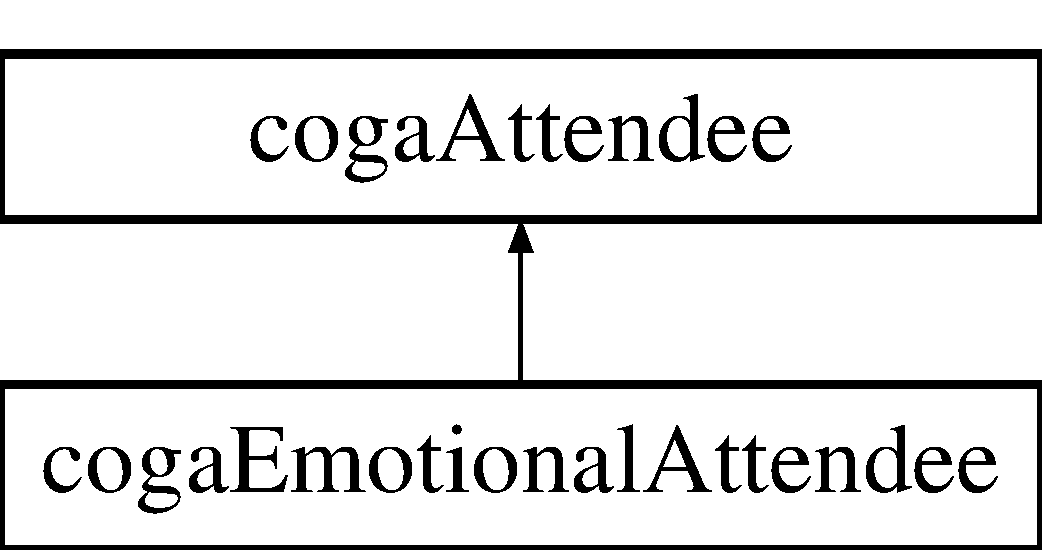
\includegraphics[height=2.000000cm]{classcoga_attendee}
\end{center}
\end{figure}
\subsection*{\-Public \-Member \-Functions}
\begin{DoxyCompactItemize}
\item 
\hypertarget{classcoga_attendee_a5e52181e3f89aa3984d7557723bad7f7}{
{\bfseries coga\-Attendee} (int \-I\-D=0)}
\label{classcoga_attendee_a5e52181e3f89aa3984d7557723bad7f7}

\item 
\hypertarget{classcoga_attendee_a62daed668f89a2ef922d66028497175b}{
virtual void {\bfseries set\-Name} (std\-::string name)=0}
\label{classcoga_attendee_a62daed668f89a2ef922d66028497175b}

\item 
\hypertarget{classcoga_attendee_addf8c2744080cc33e0cb1772b9c2eca7}{
virtual std\-::string {\bfseries get\-Name} ()}
\label{classcoga_attendee_addf8c2744080cc33e0cb1772b9c2eca7}

\item 
\hypertarget{classcoga_attendee_a087404bec069467c4e956a3463ba267d}{
virtual void {\bfseries set\-Local\-I\-D} (int id)}
\label{classcoga_attendee_a087404bec069467c4e956a3463ba267d}

\item 
\hypertarget{classcoga_attendee_ab67a78cce68214cb860ab79ecdd8045d}{
virtual int {\bfseries get\-Local\-I\-D} ()}
\label{classcoga_attendee_ab67a78cce68214cb860ab79ecdd8045d}

\item 
\hypertarget{classcoga_attendee_a0a2a69e948ab07b78d27abeeb962cb36}{
virtual std\-::string {\bfseries get\-Global\-I\-D} ()}
\label{classcoga_attendee_a0a2a69e948ab07b78d27abeeb962cb36}

\item 
\hypertarget{classcoga_attendee_ab9e63e1232ce77ad2d5f19019521be2a}{
virtual void {\bfseries set\-Global\-I\-D} (std\-::string new\-Global\-I\-D)=0}
\label{classcoga_attendee_ab9e63e1232ce77ad2d5f19019521be2a}

\end{DoxyCompactItemize}
\subsection*{\-Protected \-Attributes}
\begin{DoxyCompactItemize}
\item 
\hypertarget{classcoga_attendee_a04ed9ade71e96aefe7b9b6d261b6d139}{
std\-::string {\bfseries \-\_\-name}}
\label{classcoga_attendee_a04ed9ade71e96aefe7b9b6d261b6d139}

\item 
\hypertarget{classcoga_attendee_a17e66f5268ca061547f2306f20e7709c}{
int {\bfseries local\-I\-D}}
\label{classcoga_attendee_a17e66f5268ca061547f2306f20e7709c}

\item 
\hypertarget{classcoga_attendee_aa3aa7163f1e63993a84130f18b0cdaea}{
std\-::string {\bfseries global\-I\-D}}
\label{classcoga_attendee_aa3aa7163f1e63993a84130f18b0cdaea}

\end{DoxyCompactItemize}


\subsection{\-Detailed \-Description}


\-Definition at line 32 of file coga\-Attendee.\-h.



\-The documentation for this class was generated from the following files\-:\begin{DoxyCompactItemize}
\item 
coga\-Attendee.\-h\item 
coga\-Attendee.\-cc\end{DoxyCompactItemize}

\hypertarget{classcoga_emotional_attendee}{
\section{coga\-Emotional\-Attendee \-Class \-Reference}
\label{classcoga_emotional_attendee}\index{coga\-Emotional\-Attendee@{coga\-Emotional\-Attendee}}
}
\-Inheritance diagram for coga\-Emotional\-Attendee\-:\begin{figure}[H]
\begin{center}
\leavevmode
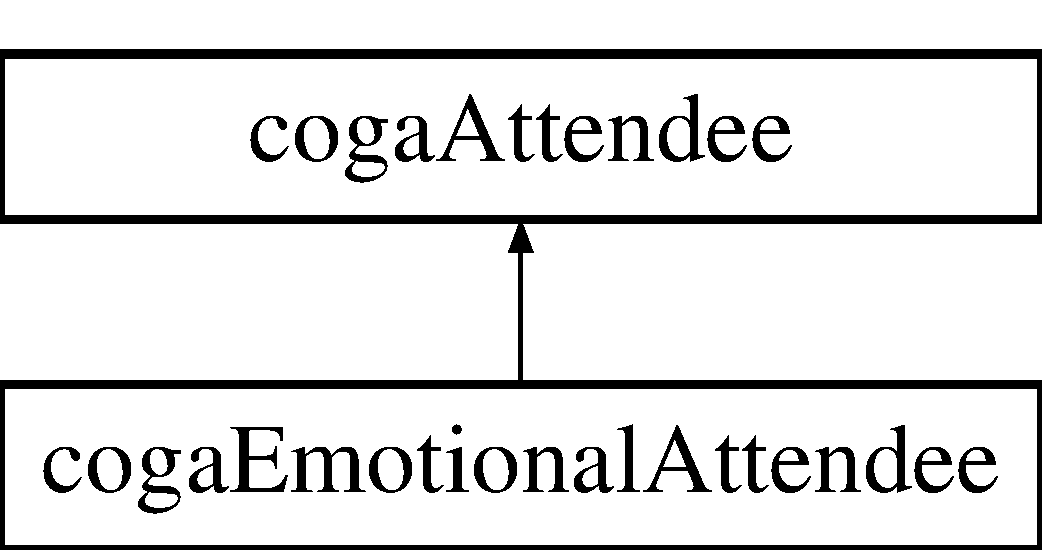
\includegraphics[height=2.000000cm]{classcoga_emotional_attendee}
\end{center}
\end{figure}
\subsection*{\-Public \-Member \-Functions}
\begin{DoxyCompactItemize}
\item 
\hypertarget{classcoga_emotional_attendee_a39576b6dd36019afd7d0caedfeaeedeb}{
{\bfseries coga\-Emotional\-Attendee} (int \-I\-D=0)}
\label{classcoga_emotional_attendee_a39576b6dd36019afd7d0caedfeaeedeb}

\item 
\hypertarget{classcoga_emotional_attendee_abc69dd68e0f9643f83df03d640ec66b5}{
int {\bfseries get\-X\-Pos} ()}
\label{classcoga_emotional_attendee_abc69dd68e0f9643f83df03d640ec66b5}

\item 
\hypertarget{classcoga_emotional_attendee_af954386831fd92696135fae2537daa9d}{
int {\bfseries get\-Y\-Pos} ()}
\label{classcoga_emotional_attendee_af954386831fd92696135fae2537daa9d}

\item 
\hypertarget{classcoga_emotional_attendee_a87d9487fd2692bab6cd1e7e9adff4a66}{
int {\bfseries get\-Z\-Pos} ()}
\label{classcoga_emotional_attendee_a87d9487fd2692bab6cd1e7e9adff4a66}

\item 
\hypertarget{classcoga_emotional_attendee_aec58012485bb81377b12116010c7b382}{
int {\bfseries get\-X\-Tens} ()}
\label{classcoga_emotional_attendee_aec58012485bb81377b12116010c7b382}

\item 
\hypertarget{classcoga_emotional_attendee_a46ee0866dc001df2154fa4ff26672a71}{
int {\bfseries get\-Y\-Tens} ()}
\label{classcoga_emotional_attendee_a46ee0866dc001df2154fa4ff26672a71}

\item 
\hypertarget{classcoga_emotional_attendee_a24ad1cd91a788c988de9d5ab825cdf7b}{
int {\bfseries get\-Slope} ()}
\label{classcoga_emotional_attendee_a24ad1cd91a788c988de9d5ab825cdf7b}

\item 
\hypertarget{classcoga_emotional_attendee_a80b5b80f14e3781b439bc4060af637e5}{
int {\bfseries get\-Mass} ()}
\label{classcoga_emotional_attendee_a80b5b80f14e3781b439bc4060af637e5}

\item 
\hypertarget{classcoga_emotional_attendee_a99353cb7284ab122cb843a8060e6606a}{
int {\bfseries get\-Alpha} ()}
\label{classcoga_emotional_attendee_a99353cb7284ab122cb843a8060e6606a}

\item 
\hypertarget{classcoga_emotional_attendee_aee89d85fadfb7bd51c2c69ad44ab1fe8}{
int {\bfseries get\-Beta} ()}
\label{classcoga_emotional_attendee_aee89d85fadfb7bd51c2c69ad44ab1fe8}

\item 
\hypertarget{classcoga_emotional_attendee_ab6b912a8b35900ab7bf7aea32b7ece04}{
int {\bfseries get\-Factor} ()}
\label{classcoga_emotional_attendee_ab6b912a8b35900ab7bf7aea32b7ece04}

\item 
\hypertarget{classcoga_emotional_attendee_a18b4811afb2e9f0ab7927a4a776bbeb0}{
int {\bfseries get\-Update\-Rate} ()}
\label{classcoga_emotional_attendee_a18b4811afb2e9f0ab7927a4a776bbeb0}

\item 
\hypertarget{classcoga_emotional_attendee_af3c5f2f6dbb95df16c74255eaf6bda54}{
int {\bfseries get\-P\-Value} ()}
\label{classcoga_emotional_attendee_af3c5f2f6dbb95df16c74255eaf6bda54}

\item 
\hypertarget{classcoga_emotional_attendee_a244c4c5c5fc242d9a36efd3ebb771398}{
int {\bfseries get\-A\-Value} ()}
\label{classcoga_emotional_attendee_a244c4c5c5fc242d9a36efd3ebb771398}

\item 
\hypertarget{classcoga_emotional_attendee_ad272c1b77f55c241455ed287d35b6c77}{
int {\bfseries get\-D\-Value} ()}
\label{classcoga_emotional_attendee_ad272c1b77f55c241455ed287d35b6c77}

\item 
\hypertarget{classcoga_emotional_attendee_abe31206754bad856297e3b97acaeb3a6}{
void {\bfseries set\-X\-Pos} (int xpos)}
\label{classcoga_emotional_attendee_abe31206754bad856297e3b97acaeb3a6}

\item 
\hypertarget{classcoga_emotional_attendee_a120445191812ae3afc6d34e07c5a8309}{
void {\bfseries set\-Y\-Pos} (int ypos)}
\label{classcoga_emotional_attendee_a120445191812ae3afc6d34e07c5a8309}

\item 
\hypertarget{classcoga_emotional_attendee_a1e96dff3dcaecc5ab2b38c147e2590b4}{
void {\bfseries set\-Z\-Pos} (int zpos)}
\label{classcoga_emotional_attendee_a1e96dff3dcaecc5ab2b38c147e2590b4}

\item 
\hypertarget{classcoga_emotional_attendee_aac7797ecddb0933f6beb7024fef5b966}{
void {\bfseries set\-P\-Value} (int pval)}
\label{classcoga_emotional_attendee_aac7797ecddb0933f6beb7024fef5b966}

\item 
\hypertarget{classcoga_emotional_attendee_a8e6f2bcaa4b867a67121f1759d7c18f8}{
void {\bfseries set\-A\-Value} (int aval)}
\label{classcoga_emotional_attendee_a8e6f2bcaa4b867a67121f1759d7c18f8}

\item 
\hypertarget{classcoga_emotional_attendee_a06f18eda6c9256f4b4e65209796a3304}{
void {\bfseries set\-D\-Value} (int dval)}
\label{classcoga_emotional_attendee_a06f18eda6c9256f4b4e65209796a3304}

\item 
\hypertarget{classcoga_emotional_attendee_a1bbb916265b90b4fb10a20bb306a082b}{
void {\bfseries set\-Slope} (int sval)}
\label{classcoga_emotional_attendee_a1bbb916265b90b4fb10a20bb306a082b}

\item 
\hypertarget{classcoga_emotional_attendee_a157adcc4e70d7135d8c6d29486338003}{
void {\bfseries set\-Mass} (int mval)}
\label{classcoga_emotional_attendee_a157adcc4e70d7135d8c6d29486338003}

\item 
\hypertarget{classcoga_emotional_attendee_a9c8fbe9e1d366e29b9cb3cbd2010519b}{
void {\bfseries set\-Alpha} (int aval)}
\label{classcoga_emotional_attendee_a9c8fbe9e1d366e29b9cb3cbd2010519b}

\item 
\hypertarget{classcoga_emotional_attendee_a69334d4d7b6d7be1ce77f064a98faf60}{
void {\bfseries set\-Beta} (int bval)}
\label{classcoga_emotional_attendee_a69334d4d7b6d7be1ce77f064a98faf60}

\item 
\hypertarget{classcoga_emotional_attendee_ab343dafec638db9f4890a98f2bfd5978}{
void {\bfseries set\-Factor} (int fval)}
\label{classcoga_emotional_attendee_ab343dafec638db9f4890a98f2bfd5978}

\item 
\hypertarget{classcoga_emotional_attendee_ab18e4763c38e0097921992ac66d9960b}{
void {\bfseries set\-X\-Tens} (int xtens)}
\label{classcoga_emotional_attendee_ab18e4763c38e0097921992ac66d9960b}

\item 
\hypertarget{classcoga_emotional_attendee_a0f5c6fbccbe782eb943c75e1dd537697}{
void {\bfseries set\-Y\-Tens} (int ytens)}
\label{classcoga_emotional_attendee_a0f5c6fbccbe782eb943c75e1dd537697}

\item 
\hypertarget{classcoga_emotional_attendee_ae2cd890c29e3668e30918429376d0ae7}{
void {\bfseries set\-Update\-Rate} (int update\-Rate)}
\label{classcoga_emotional_attendee_ae2cd890c29e3668e30918429376d0ae7}

\item 
\hypertarget{classcoga_emotional_attendee_afc12eba3c96bd738624c6994cc6bce1a}{
void {\bfseries set\-Name} (std\-::string name)}
\label{classcoga_emotional_attendee_afc12eba3c96bd738624c6994cc6bce1a}

\item 
\hypertarget{classcoga_emotional_attendee_a45a361be78e01c06bc3ce4048d85eb77}{
void {\bfseries set\-Global\-I\-D} (std\-::string new\-Global\-I\-D)}
\label{classcoga_emotional_attendee_a45a361be78e01c06bc3ce4048d85eb77}

\item 
void \hyperlink{classcoga_emotional_attendee_a1e9cb2beb83ee9ff9efe7d4431ab464c}{update\-P\-A\-Dstring} ()
\item 
\hypertarget{classcoga_emotional_attendee_a7584cc6606dafad50180400abaa12804}{
void {\bfseries do\-Mapping} ()}
\label{classcoga_emotional_attendee_a7584cc6606dafad50180400abaa12804}

\item 
\hypertarget{classcoga_emotional_attendee_a02677bbe04c2bc25673fa9b596091a07}{
bool {\bfseries update} ()}
\label{classcoga_emotional_attendee_a02677bbe04c2bc25673fa9b596091a07}

\item 
\hypertarget{classcoga_emotional_attendee_a195881d129cd436ee355610953096122}{
void {\bfseries reset\-Forces} ()}
\label{classcoga_emotional_attendee_a195881d129cd436ee355610953096122}

\end{DoxyCompactItemize}
\subsection*{\-Public \-Attributes}
\begin{DoxyCompactItemize}
\item 
\hypertarget{classcoga_emotional_attendee_a3e6e692655b7802271a55ebb56ced690}{
std\-::string {\bfseries \-P\-A\-Dstring}}
\label{classcoga_emotional_attendee_a3e6e692655b7802271a55ebb56ced690}

\item 
\hypertarget{classcoga_emotional_attendee_a38d3bc46bb4969a9a59f5034a1337b5c}{
std\-::string {\bfseries \-P\-A\-Dstring\-\_\-last}}
\label{classcoga_emotional_attendee_a38d3bc46bb4969a9a59f5034a1337b5c}

\item 
\hypertarget{classcoga_emotional_attendee_a930cc5f296d7b97815dcb9eecd197913}{
\hyperlink{class_emotion_dynamics}{\-Emotion\-Dynamics} $\ast$ {\bfseries \-Emo\-Con\-Person}}
\label{classcoga_emotional_attendee_a930cc5f296d7b97815dcb9eecd197913}

\item 
\hypertarget{classcoga_emotional_attendee_aa65ba503eef10077b9f2f0b2d234c41b}{
\hyperlink{class_emotion_converter_p_a_d}{\-Emotion\-Converter\-P\-A\-D} $\ast$ {\bfseries \-P\-A\-Dconverter}}
\label{classcoga_emotional_attendee_aa65ba503eef10077b9f2f0b2d234c41b}

\item 
\hypertarget{classcoga_emotional_attendee_ad105ae15afcd726402f64917f4aaa8d7}{
bool {\bfseries simulation\-On}}
\label{classcoga_emotional_attendee_ad105ae15afcd726402f64917f4aaa8d7}

\end{DoxyCompactItemize}


\subsection{\-Detailed \-Description}


\-Definition at line 34 of file coga\-Emotional\-Attendee.\-h.



\subsection{\-Member \-Function \-Documentation}
\hypertarget{classcoga_emotional_attendee_a1e9cb2beb83ee9ff9efe7d4431ab464c}{
\index{coga\-Emotional\-Attendee@{coga\-Emotional\-Attendee}!update\-P\-A\-Dstring@{update\-P\-A\-Dstring}}
\index{update\-P\-A\-Dstring@{update\-P\-A\-Dstring}!cogaEmotionalAttendee@{coga\-Emotional\-Attendee}}
\subsubsection[{update\-P\-A\-Dstring}]{\setlength{\rightskip}{0pt plus 5cm}void coga\-Emotional\-Attendee\-::update\-P\-A\-Dstring (
\begin{DoxyParamCaption}
{}
\end{DoxyParamCaption}
)}}
\label{classcoga_emotional_attendee_a1e9cb2beb83ee9ff9efe7d4431ab464c}
\-Hier wird bei einer \-Ver�nderung des \-P\-A\-Dstrings das '\-Max sagt\-: ...' aktualisiert.\par
 

\-Definition at line 286 of file coga\-Emotional\-Attendee.\-cc.



\-The documentation for this class was generated from the following files\-:\begin{DoxyCompactItemize}
\item 
coga\-Emotional\-Attendee.\-h\item 
coga\-Emotional\-Attendee.\-cc\end{DoxyCompactItemize}

\hypertarget{class_emo_pos2_reach}{
\section{\-Emo\-Pos2\-Reach \-Class \-Reference}
\label{class_emo_pos2_reach}\index{\-Emo\-Pos2\-Reach@{\-Emo\-Pos2\-Reach}}
}


{\ttfamily \#include $<$\-Emotion\-Container.\-h$>$}

\subsection*{\-Public \-Member \-Functions}
\begin{DoxyCompactItemize}
\item 
\hyperlink{class_emo_pos2_reach_a8b150d60a80a759dc33f4ca52c7649f9}{\-Emo\-Pos2\-Reach} ()
\item 
\hypertarget{class_emo_pos2_reach_a73b3bd1eefbcdc5993dd19bddd3de0c1}{
{\bfseries \-Emo\-Pos2\-Reach} (const \hyperlink{class_emo_pos2_reach}{\-Emo\-Pos2\-Reach} \&emo\-Pos)}
\label{class_emo_pos2_reach_a73b3bd1eefbcdc5993dd19bddd3de0c1}

\item 
virtual \hyperlink{class_emo_pos2_reach_a59695111d41f3c0b7ebb0651f2d3a167}{$\sim$\-Emo\-Pos2\-Reach} ()
\item 
int \hyperlink{class_emo_pos2_reach_ac39da00fcf926534ad515d58b4655261}{get\-X\-Pos2\-Reach} ()
\item 
int \hyperlink{class_emo_pos2_reach_ae5c96309806115ebf1d4c89a072967c6}{get\-Y\-Pos2\-Reach} ()
\item 
void \hyperlink{class_emo_pos2_reach_a8c5472952913fd39881cb7c8306bb039}{set\-Positions2\-Reach} (int x\-Pos, int y\-Pos)
\item 
void \hyperlink{class_emo_pos2_reach_acd0790143f40a33195ffc62e146fa3b0}{set\-X\-Valid} (bool valid)
\item 
void \hyperlink{class_emo_pos2_reach_a57cc4adbba8486f1b27ca171ed3bd80d}{set\-Y\-Valid} (bool valid)
\item 
bool \hyperlink{class_emo_pos2_reach_aa500036b5172705a162467fffd9216eb}{get\-X\-Valid} ()
\item 
bool \hyperlink{class_emo_pos2_reach_a844aaa86d9adf370d8bef6387fd12e44}{get\-Y\-Valid} ()
\end{DoxyCompactItemize}
\subsection*{\-Protected \-Attributes}
\begin{DoxyCompactItemize}
\item 
\hypertarget{class_emo_pos2_reach_ad3380cde20548f21d1f09f6f14fe192b}{
int {\bfseries x\-Pos2\-Reach}}
\label{class_emo_pos2_reach_ad3380cde20548f21d1f09f6f14fe192b}

\item 
\hypertarget{class_emo_pos2_reach_ad8fea368615381740df1384e1f70a46c}{
int {\bfseries y\-Pos2\-Reach}}
\label{class_emo_pos2_reach_ad8fea368615381740df1384e1f70a46c}

\item 
\hypertarget{class_emo_pos2_reach_a76954287470ee07954f244edffb7684a}{
bool {\bfseries x\-Valid}}
\label{class_emo_pos2_reach_a76954287470ee07954f244edffb7684a}

\item 
\hypertarget{class_emo_pos2_reach_abf24b7a70757bea15fe96d48ca597387}{
bool {\bfseries y\-Valid}}
\label{class_emo_pos2_reach_abf24b7a70757bea15fe96d48ca597387}

\end{DoxyCompactItemize}


\subsection{\-Detailed \-Description}
\-Container-\/\-Klasse fuer die \-Position, die im \-Dynamik-\/\-Raum erreicht werden soll. \-Hier wird die \-Gueltigkeit der \-Koordinaten verwaltet. 

\-Definition at line 40 of file \-Emotion\-Container.\-h.



\subsection{\-Constructor \& \-Destructor \-Documentation}
\hypertarget{class_emo_pos2_reach_a8b150d60a80a759dc33f4ca52c7649f9}{
\index{\-Emo\-Pos2\-Reach@{\-Emo\-Pos2\-Reach}!\-Emo\-Pos2\-Reach@{\-Emo\-Pos2\-Reach}}
\index{\-Emo\-Pos2\-Reach@{\-Emo\-Pos2\-Reach}!EmoPos2Reach@{\-Emo\-Pos2\-Reach}}
\subsubsection[{\-Emo\-Pos2\-Reach}]{\setlength{\rightskip}{0pt plus 5cm}\-Emo\-Pos2\-Reach\-::\-Emo\-Pos2\-Reach (
\begin{DoxyParamCaption}
{}
\end{DoxyParamCaption}
)}}
\label{class_emo_pos2_reach_a8b150d60a80a759dc33f4ca52c7649f9}
\-Setzt x\-Pos2\-Reach und y\-Pos2\-Reach auf 0, booleans auf false 

\-Definition at line 38 of file \-Emotion\-Container.\-cc.

\hypertarget{class_emo_pos2_reach_a59695111d41f3c0b7ebb0651f2d3a167}{
\index{\-Emo\-Pos2\-Reach@{\-Emo\-Pos2\-Reach}!$\sim$\-Emo\-Pos2\-Reach@{$\sim$\-Emo\-Pos2\-Reach}}
\index{$\sim$\-Emo\-Pos2\-Reach@{$\sim$\-Emo\-Pos2\-Reach}!EmoPos2Reach@{\-Emo\-Pos2\-Reach}}
\subsubsection[{$\sim$\-Emo\-Pos2\-Reach}]{\setlength{\rightskip}{0pt plus 5cm}\-Emo\-Pos2\-Reach\-::$\sim$\-Emo\-Pos2\-Reach (
\begin{DoxyParamCaption}
{}
\end{DoxyParamCaption}
)\hspace{0.3cm}{\ttfamily  \mbox{[}virtual\mbox{]}}}}
\label{class_emo_pos2_reach_a59695111d41f3c0b7ebb0651f2d3a167}
nichts 

\-Definition at line 55 of file \-Emotion\-Container.\-cc.



\subsection{\-Member \-Function \-Documentation}
\hypertarget{class_emo_pos2_reach_ac39da00fcf926534ad515d58b4655261}{
\index{\-Emo\-Pos2\-Reach@{\-Emo\-Pos2\-Reach}!get\-X\-Pos2\-Reach@{get\-X\-Pos2\-Reach}}
\index{get\-X\-Pos2\-Reach@{get\-X\-Pos2\-Reach}!EmoPos2Reach@{\-Emo\-Pos2\-Reach}}
\subsubsection[{get\-X\-Pos2\-Reach}]{\setlength{\rightskip}{0pt plus 5cm}int \-Emo\-Pos2\-Reach\-::get\-X\-Pos2\-Reach (
\begin{DoxyParamCaption}
{}
\end{DoxyParamCaption}
)}}
\label{class_emo_pos2_reach_ac39da00fcf926534ad515d58b4655261}
returns the x position target 

\-Definition at line 63 of file \-Emotion\-Container.\-cc.

\hypertarget{class_emo_pos2_reach_aa500036b5172705a162467fffd9216eb}{
\index{\-Emo\-Pos2\-Reach@{\-Emo\-Pos2\-Reach}!get\-X\-Valid@{get\-X\-Valid}}
\index{get\-X\-Valid@{get\-X\-Valid}!EmoPos2Reach@{\-Emo\-Pos2\-Reach}}
\subsubsection[{get\-X\-Valid}]{\setlength{\rightskip}{0pt plus 5cm}bool \-Emo\-Pos2\-Reach\-::get\-X\-Valid (
\begin{DoxyParamCaption}
{}
\end{DoxyParamCaption}
)}}
\label{class_emo_pos2_reach_aa500036b5172705a162467fffd9216eb}
\-Checks validity of x 

\-Definition at line 99 of file \-Emotion\-Container.\-cc.

\hypertarget{class_emo_pos2_reach_ae5c96309806115ebf1d4c89a072967c6}{
\index{\-Emo\-Pos2\-Reach@{\-Emo\-Pos2\-Reach}!get\-Y\-Pos2\-Reach@{get\-Y\-Pos2\-Reach}}
\index{get\-Y\-Pos2\-Reach@{get\-Y\-Pos2\-Reach}!EmoPos2Reach@{\-Emo\-Pos2\-Reach}}
\subsubsection[{get\-Y\-Pos2\-Reach}]{\setlength{\rightskip}{0pt plus 5cm}int \-Emo\-Pos2\-Reach\-::get\-Y\-Pos2\-Reach (
\begin{DoxyParamCaption}
{}
\end{DoxyParamCaption}
)}}
\label{class_emo_pos2_reach_ae5c96309806115ebf1d4c89a072967c6}
returns the y position target 

\-Definition at line 72 of file \-Emotion\-Container.\-cc.

\hypertarget{class_emo_pos2_reach_a844aaa86d9adf370d8bef6387fd12e44}{
\index{\-Emo\-Pos2\-Reach@{\-Emo\-Pos2\-Reach}!get\-Y\-Valid@{get\-Y\-Valid}}
\index{get\-Y\-Valid@{get\-Y\-Valid}!EmoPos2Reach@{\-Emo\-Pos2\-Reach}}
\subsubsection[{get\-Y\-Valid}]{\setlength{\rightskip}{0pt plus 5cm}bool \-Emo\-Pos2\-Reach\-::get\-Y\-Valid (
\begin{DoxyParamCaption}
{}
\end{DoxyParamCaption}
)}}
\label{class_emo_pos2_reach_a844aaa86d9adf370d8bef6387fd12e44}
\-Checks validity of y 

\-Definition at line 108 of file \-Emotion\-Container.\-cc.

\hypertarget{class_emo_pos2_reach_a8c5472952913fd39881cb7c8306bb039}{
\index{\-Emo\-Pos2\-Reach@{\-Emo\-Pos2\-Reach}!set\-Positions2\-Reach@{set\-Positions2\-Reach}}
\index{set\-Positions2\-Reach@{set\-Positions2\-Reach}!EmoPos2Reach@{\-Emo\-Pos2\-Reach}}
\subsubsection[{set\-Positions2\-Reach}]{\setlength{\rightskip}{0pt plus 5cm}void \-Emo\-Pos2\-Reach\-::set\-Positions2\-Reach (
\begin{DoxyParamCaption}
\item[{int}]{x\-Pos, }
\item[{int}]{y\-Pos}
\end{DoxyParamCaption}
)}}
\label{class_emo_pos2_reach_a8c5472952913fd39881cb7c8306bb039}
\-Keeps track of limits 

\-Definition at line 81 of file \-Emotion\-Container.\-cc.

\hypertarget{class_emo_pos2_reach_acd0790143f40a33195ffc62e146fa3b0}{
\index{\-Emo\-Pos2\-Reach@{\-Emo\-Pos2\-Reach}!set\-X\-Valid@{set\-X\-Valid}}
\index{set\-X\-Valid@{set\-X\-Valid}!EmoPos2Reach@{\-Emo\-Pos2\-Reach}}
\subsubsection[{set\-X\-Valid}]{\setlength{\rightskip}{0pt plus 5cm}void \-Emo\-Pos2\-Reach\-::set\-X\-Valid (
\begin{DoxyParamCaption}
\item[{bool}]{valid}
\end{DoxyParamCaption}
)}}
\label{class_emo_pos2_reach_acd0790143f40a33195ffc62e146fa3b0}
\-Setzt x\-Valid. 

\-Definition at line 117 of file \-Emotion\-Container.\-cc.

\hypertarget{class_emo_pos2_reach_a57cc4adbba8486f1b27ca171ed3bd80d}{
\index{\-Emo\-Pos2\-Reach@{\-Emo\-Pos2\-Reach}!set\-Y\-Valid@{set\-Y\-Valid}}
\index{set\-Y\-Valid@{set\-Y\-Valid}!EmoPos2Reach@{\-Emo\-Pos2\-Reach}}
\subsubsection[{set\-Y\-Valid}]{\setlength{\rightskip}{0pt plus 5cm}void \-Emo\-Pos2\-Reach\-::set\-Y\-Valid (
\begin{DoxyParamCaption}
\item[{bool}]{valid}
\end{DoxyParamCaption}
)}}
\label{class_emo_pos2_reach_a57cc4adbba8486f1b27ca171ed3bd80d}
\-Setzt y\-Valid. 

\-Definition at line 126 of file \-Emotion\-Container.\-cc.



\-The documentation for this class was generated from the following files\-:\begin{DoxyCompactItemize}
\item 
\-Emotion\-Container.\-h\item 
\-Emotion\-Container.\-cc\end{DoxyCompactItemize}

\hypertarget{class_emotion_container}{
\section{\-Emotion\-Container \-Class \-Reference}
\label{class_emotion_container}\index{\-Emotion\-Container@{\-Emotion\-Container}}
}


{\ttfamily \#include $<$\-Emotion\-Container.\-h$>$}

\-Inheritance diagram for \-Emotion\-Container\-:\begin{figure}[H]
\begin{center}
\leavevmode
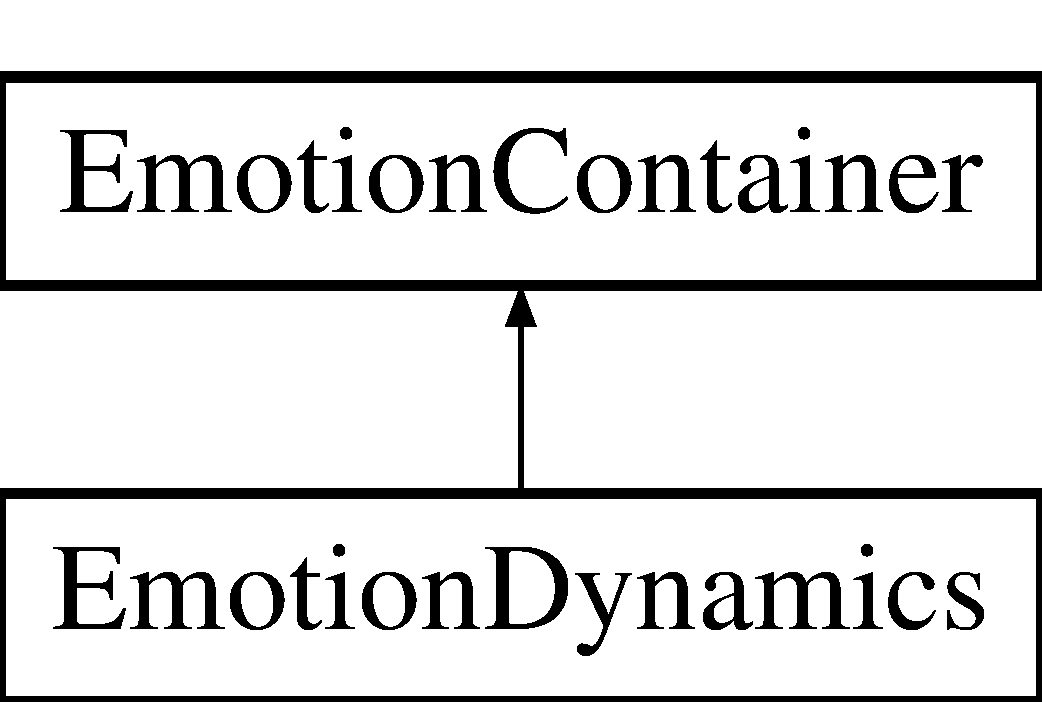
\includegraphics[height=2.000000cm]{class_emotion_container}
\end{center}
\end{figure}
\subsection*{\-Public \-Member \-Functions}
\begin{DoxyCompactItemize}
\item 
\hyperlink{class_emotion_container_a0cd2f36521f30b93582231d00c3ee8e9}{\-Emotion\-Container} ()
\item 
\hyperlink{class_emotion_container_ab47c17d4f7ce7d862fdf278d7878bdcf}{\-Emotion\-Container} (const \hyperlink{class_emotion_container}{\-Emotion\-Container} \&emo\-Con)
\item 
\hypertarget{class_emotion_container_a70d9dd45542e029d4eba3dcbddf1b717}{
virtual void {\bfseries write\-Transferable} (std\-::ostream \&ostr) const }
\label{class_emotion_container_a70d9dd45542e029d4eba3dcbddf1b717}

\item 
\hypertarget{class_emotion_container_a33d17071e475f57c9856f69464eb4db5}{
virtual void {\bfseries read\-Transferable} (std\-::istream \&)}
\label{class_emotion_container_a33d17071e475f57c9856f69464eb4db5}

\item 
virtual void \hyperlink{class_emotion_container_a8c63f4c9e9c558b4cecdf1aab9c81bd0}{update} (float \-\_\-dt)
\item 
\hypertarget{class_emotion_container_a962cd6110a2793a2d5c4582ad0904b78}{
virtual void {\bfseries init} ()}
\label{class_emotion_container_a962cd6110a2793a2d5c4582ad0904b78}

\item 
\hypertarget{class_emotion_container_abd39cb9d11335f30eff2392f93b73a3d}{
std\-::string {\bfseries get\-Type} ()}
\label{class_emotion_container_abd39cb9d11335f30eff2392f93b73a3d}

\item 
\hypertarget{class_emotion_container_a547c9f7cde3d3408ea0811a28395e3e8}{
\-A\-S\-Vector\-M\-Map {\bfseries get\-Affect\-Likelihoods} ()}
\label{class_emotion_container_a547c9f7cde3d3408ea0811a28395e3e8}

\item 
\hypertarget{class_emotion_container_a628c9fcecdf630c159c336b6197a2134}{
\hyperlink{class_affective_state}{\-Affective\-State} $\ast$ {\bfseries get\-Affective\-State\-By\-Type} (std\-::string type)}
\label{class_emotion_container_a628c9fcecdf630c159c336b6197a2134}

\item 
\hypertarget{class_emotion_container_a5a1cf35a1c16bae3d44ce4311256994c}{
void {\bfseries dump\-Affective\-States} (std\-::ostream \&ostr)}
\label{class_emotion_container_a5a1cf35a1c16bae3d44ce4311256994c}

\item 
\hypertarget{class_emotion_container_a3222476a63c2f978a29d416b7da1d1a3}{
int {\bfseries get\-A\-S\-Id} (std\-::string emotionclass=\char`\"{}any\char`\"{})}
\label{class_emotion_container_a3222476a63c2f978a29d416b7da1d1a3}

\item 
\hypertarget{class_emotion_container_a2a62a951674e48c4fc7e5721ee8eb5c4}{
std\-::string {\bfseries get\-A\-S\-Type} (std\-::string emotionclass=\char`\"{}any\char`\"{})}
\label{class_emotion_container_a2a62a951674e48c4fc7e5721ee8eb5c4}

\item 
\hypertarget{class_emotion_container_aef8c2ba099d035998c90383fece30e20}{
float {\bfseries get\-A\-S\-Likelihood} (std\-::string emotionclass=\char`\"{}any\char`\"{})}
\label{class_emotion_container_aef8c2ba099d035998c90383fece30e20}

\item 
\hypertarget{class_emotion_container_a7b6b49c2ec038157fee83e1f7c6afc51}{
bool {\bfseries is\-Active} ()}
\label{class_emotion_container_a7b6b49c2ec038157fee83e1f7c6afc51}

\item 
\hypertarget{class_emotion_container_a8edcf7d2c76e3a49d09f4cb1ea1b6c43}{
bool {\bfseries trigger\-A\-S} (std\-::string \-\_\-type, double new\-Lifetime=-\/1.\-0)}
\label{class_emotion_container_a8edcf7d2c76e3a49d09f4cb1ea1b6c43}

\item 
void \hyperlink{class_emotion_container_a2438c1f0119baf3f3df140f246d50783}{update\-Affect\-Likelihoods} (bool force\-P\-A\-Dupdate=false)
\end{DoxyCompactItemize}
\subsection*{\-Public \-Attributes}
\begin{DoxyCompactItemize}
\item 
\hypertarget{class_emotion_container_af50ab9b2b4955a337b9659ce4f795fed}{
double {\bfseries dt}}
\label{class_emotion_container_af50ab9b2b4955a337b9659ce4f795fed}

\item 
\hypertarget{class_emotion_container_ac84d0dcd287bce8986c76e84bd46bbd9}{
std\-::vector$<$ \hyperlink{class_affective_state}{\-Affective\-State} $\ast$ $>$ {\bfseries affective\-States}}
\label{class_emotion_container_ac84d0dcd287bce8986c76e84bd46bbd9}

\item 
\hypertarget{class_emotion_container_af004404f7cf8b28c0be3b6875fda153a}{
\-Affect\-Type\-Likelihoods\-M\-Map {\bfseries atlmmap}}
\label{class_emotion_container_af004404f7cf8b28c0be3b6875fda153a}

\end{DoxyCompactItemize}
\subsection*{\-Protected \-Member \-Functions}
\begin{DoxyCompactItemize}
\item 
\hypertarget{class_emotion_container_ae4ab08ca4de2ee7cbbdd6178e38dc560}{
bool {\bfseries build\-Primary\-Emotion} (std\-::vector$<$ float $>$ v, std\-::string type, std\-::string decay\-Func)}
\label{class_emotion_container_ae4ab08ca4de2ee7cbbdd6178e38dc560}

\item 
\hypertarget{class_emotion_container_aa280b192728fd4ab900fd6ce8792a995}{
bool {\bfseries build\-Secondary\-Emotion} (std\-::string secfilename)}
\label{class_emotion_container_aa280b192728fd4ab900fd6ce8792a995}

\end{DoxyCompactItemize}
\subsection*{\-Protected \-Attributes}
\begin{DoxyCompactItemize}
\item 
\hypertarget{class_emotion_container_a55a74daa41036de8653c9d9c92894544}{
std\-::string {\bfseries type}}
\label{class_emotion_container_a55a74daa41036de8653c9d9c92894544}

\item 
\hypertarget{class_emotion_container_a710ccc1213bd8ee3dd9cc79efa6a129d}{
\-A\-S\-Vector\-M\-Map {\bfseries asvmmap}}
\label{class_emotion_container_a710ccc1213bd8ee3dd9cc79efa6a129d}

\item 
\hypertarget{class_emotion_container_a35dc16eeb7df5034d5a84e151ecf7edf}{
bool {\bfseries active}}
\label{class_emotion_container_a35dc16eeb7df5034d5a84e151ecf7edf}

\end{DoxyCompactItemize}
\subsection*{\-Friends}
\begin{DoxyCompactItemize}
\item 
\hypertarget{class_emotion_container_abcef228967f40c7b02f677e5fa9272fa}{
class \-W\-A\-S\-A\-B\-I\-E\-N\-G\-I\-N\-E\-S\-H\-A\-R\-E\-D\-\_\-\-E\-X\-P\-O\-R\-T {\bfseries coga\-Emotional\-Attendee}}
\label{class_emotion_container_abcef228967f40c7b02f677e5fa9272fa}

\end{DoxyCompactItemize}


\subsection{\-Detailed \-Description}
\-Diese \-Klasse kapselt alle physikalischen \-Variablen des \-Dynamik-\/\-Raumes. 

\-Definition at line 64 of file \-Emotion\-Container.\-h.



\subsection{\-Constructor \& \-Destructor \-Documentation}
\hypertarget{class_emotion_container_a0cd2f36521f30b93582231d00c3ee8e9}{
\index{\-Emotion\-Container@{\-Emotion\-Container}!\-Emotion\-Container@{\-Emotion\-Container}}
\index{\-Emotion\-Container@{\-Emotion\-Container}!EmotionContainer@{\-Emotion\-Container}}
\subsubsection[{\-Emotion\-Container}]{\setlength{\rightskip}{0pt plus 5cm}\-Emotion\-Container\-::\-Emotion\-Container (
\begin{DoxyParamCaption}
{}
\end{DoxyParamCaption}
)}}
\label{class_emotion_container_a0cd2f36521f30b93582231d00c3ee8e9}
inits the values 

\-Definition at line 134 of file \-Emotion\-Container.\-cc.

\hypertarget{class_emotion_container_ab47c17d4f7ce7d862fdf278d7878bdcf}{
\index{\-Emotion\-Container@{\-Emotion\-Container}!\-Emotion\-Container@{\-Emotion\-Container}}
\index{\-Emotion\-Container@{\-Emotion\-Container}!EmotionContainer@{\-Emotion\-Container}}
\subsubsection[{\-Emotion\-Container}]{\setlength{\rightskip}{0pt plus 5cm}\-Emotion\-Container\-::\-Emotion\-Container (
\begin{DoxyParamCaption}
\item[{const {\bf \-Emotion\-Container} \&}]{emo\-Con}
\end{DoxyParamCaption}
)}}
\label{class_emotion_container_ab47c17d4f7ce7d862fdf278d7878bdcf}
\-Simple \-Copy \-Constructor 

\-Definition at line 154 of file \-Emotion\-Container.\-cc.



\subsection{\-Member \-Function \-Documentation}
\hypertarget{class_emotion_container_a8c63f4c9e9c558b4cecdf1aab9c81bd0}{
\index{\-Emotion\-Container@{\-Emotion\-Container}!update@{update}}
\index{update@{update}!EmotionContainer@{\-Emotion\-Container}}
\subsubsection[{update}]{\setlength{\rightskip}{0pt plus 5cm}void \-Emotion\-Container\-::update (
\begin{DoxyParamCaption}
\item[{float}]{\-\_\-dt}
\end{DoxyParamCaption}
)\hspace{0.3cm}{\ttfamily  \mbox{[}virtual\mbox{]}}}}
\label{class_emotion_container_a8c63f4c9e9c558b4cecdf1aab9c81bd0}
\-We perform an update of all \-Affective\-States here, such that the intensity values are recalculated 

\-Reimplemented in \hyperlink{class_emotion_dynamics_a806fec22c1590ea3df5037bf3922a7b6}{\-Emotion\-Dynamics}.



\-Definition at line 266 of file \-Emotion\-Container.\-cc.

\hypertarget{class_emotion_container_a2438c1f0119baf3f3df140f246d50783}{
\index{\-Emotion\-Container@{\-Emotion\-Container}!update\-Affect\-Likelihoods@{update\-Affect\-Likelihoods}}
\index{update\-Affect\-Likelihoods@{update\-Affect\-Likelihoods}!EmotionContainer@{\-Emotion\-Container}}
\subsubsection[{update\-Affect\-Likelihoods}]{\setlength{\rightskip}{0pt plus 5cm}void \-Emotion\-Container\-::update\-Affect\-Likelihoods (
\begin{DoxyParamCaption}
\item[{bool}]{force\-P\-A\-Dupdate = {\ttfamily false}}
\end{DoxyParamCaption}
)}}
\label{class_emotion_container_a2438c1f0119baf3f3df140f246d50783}
\-This function returns a \-String\-Vector\-Multi\-Map with the following structure\-: \{(string type, $<$vector float$>$=\char`\"{}\char`\"{}$>$ likelihoods), ..\}, where \char`\"{}$<$vector float$>$ likelihoods\char`\"{} contains the likelihoods of every single \hyperlink{class_affect_polygon}{\-Affect\-Polygon} the \hyperlink{class_affective_state}{\-Affective\-State} \char`\"{}type\char`\"{} consists of. 

\-Definition at line 310 of file \-Emotion\-Container.\-cc.



\-The documentation for this class was generated from the following files\-:\begin{DoxyCompactItemize}
\item 
\-Emotion\-Container.\-h\item 
\-Emotion\-Container.\-cc\end{DoxyCompactItemize}

\hypertarget{class_emotion_converter}{
\section{\-Emotion\-Converter \-Class \-Reference}
\label{class_emotion_converter}\index{\-Emotion\-Converter@{\-Emotion\-Converter}}
}


{\ttfamily \#include $<$\-Emotion\-Converter.\-h$>$}

\-Inheritance diagram for \-Emotion\-Converter\-:\begin{figure}[H]
\begin{center}
\leavevmode
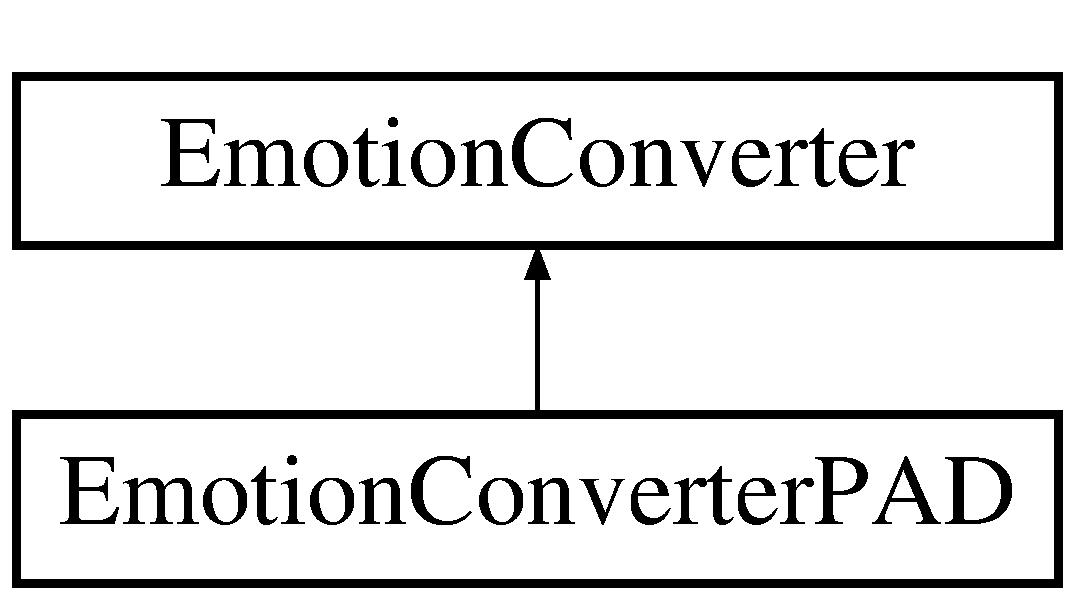
\includegraphics[height=2.000000cm]{class_emotion_converter}
\end{center}
\end{figure}
\subsection*{\-Public \-Member \-Functions}
\begin{DoxyCompactItemize}
\item 
\hyperlink{class_emotion_converter_a1a7ad7327f039f8046a7fb7f3d1f7c32}{\-Emotion\-Converter} ()
\item 
virtual \hyperlink{class_emotion_converter_ae17726b58adada29053be51ebcefd503}{$\sim$\-Emotion\-Converter} ()
\item 
\hypertarget{class_emotion_converter_a866ee18fd748c732937ed520feb1078f}{
virtual std\-::vector$<$ int $>$ {\bfseries convert\-To\-Class\-Type} (std\-::vector$<$ int $>$)=0}
\label{class_emotion_converter_a866ee18fd748c732937ed520feb1078f}

\item 
\hypertarget{class_emotion_converter_a642ea765ffebc21f73b050c18e9b17e8}{
virtual std\-::vector$<$ float $>$ {\bfseries convert\-From\-Class\-Type} (std\-::vector$<$ float $>$)=0}
\label{class_emotion_converter_a642ea765ffebc21f73b050c18e9b17e8}

\end{DoxyCompactItemize}


\subsection{\-Detailed \-Description}
\-Abstrakte \-Basisklasse fuer die \-Abbildung vom \-Dynamik-\/\-Raum in einen \-Raum zur \-Kategorisierung 

\-Definition at line 43 of file \-Emotion\-Converter.\-h.



\subsection{\-Constructor \& \-Destructor \-Documentation}
\hypertarget{class_emotion_converter_a1a7ad7327f039f8046a7fb7f3d1f7c32}{
\index{\-Emotion\-Converter@{\-Emotion\-Converter}!\-Emotion\-Converter@{\-Emotion\-Converter}}
\index{\-Emotion\-Converter@{\-Emotion\-Converter}!EmotionConverter@{\-Emotion\-Converter}}
\subsubsection[{\-Emotion\-Converter}]{\setlength{\rightskip}{0pt plus 5cm}\-Emotion\-Converter\-::\-Emotion\-Converter (
\begin{DoxyParamCaption}
{}
\end{DoxyParamCaption}
)}}
\label{class_emotion_converter_a1a7ad7327f039f8046a7fb7f3d1f7c32}
\-Leerer \-Konstruktor. 

\-Definition at line 34 of file \-Emotion\-Converter.\-cc.

\hypertarget{class_emotion_converter_ae17726b58adada29053be51ebcefd503}{
\index{\-Emotion\-Converter@{\-Emotion\-Converter}!$\sim$\-Emotion\-Converter@{$\sim$\-Emotion\-Converter}}
\index{$\sim$\-Emotion\-Converter@{$\sim$\-Emotion\-Converter}!EmotionConverter@{\-Emotion\-Converter}}
\subsubsection[{$\sim$\-Emotion\-Converter}]{\setlength{\rightskip}{0pt plus 5cm}\-Emotion\-Converter\-::$\sim$\-Emotion\-Converter (
\begin{DoxyParamCaption}
{}
\end{DoxyParamCaption}
)\hspace{0.3cm}{\ttfamily  \mbox{[}virtual\mbox{]}}}}
\label{class_emotion_converter_ae17726b58adada29053be51ebcefd503}
\-Leerer \-Destruktor. 

\-Definition at line 41 of file \-Emotion\-Converter.\-cc.



\-The documentation for this class was generated from the following files\-:\begin{DoxyCompactItemize}
\item 
\-Emotion\-Converter.\-h\item 
\-Emotion\-Converter.\-cc\end{DoxyCompactItemize}

\hypertarget{class_emotion_converter_p_a_d}{
\section{\-Emotion\-Converter\-P\-A\-D \-Class \-Reference}
\label{class_emotion_converter_p_a_d}\index{\-Emotion\-Converter\-P\-A\-D@{\-Emotion\-Converter\-P\-A\-D}}
}


{\ttfamily \#include $<$\-Emotion\-Converter.\-h$>$}

\-Inheritance diagram for \-Emotion\-Converter\-P\-A\-D\-:\begin{figure}[H]
\begin{center}
\leavevmode
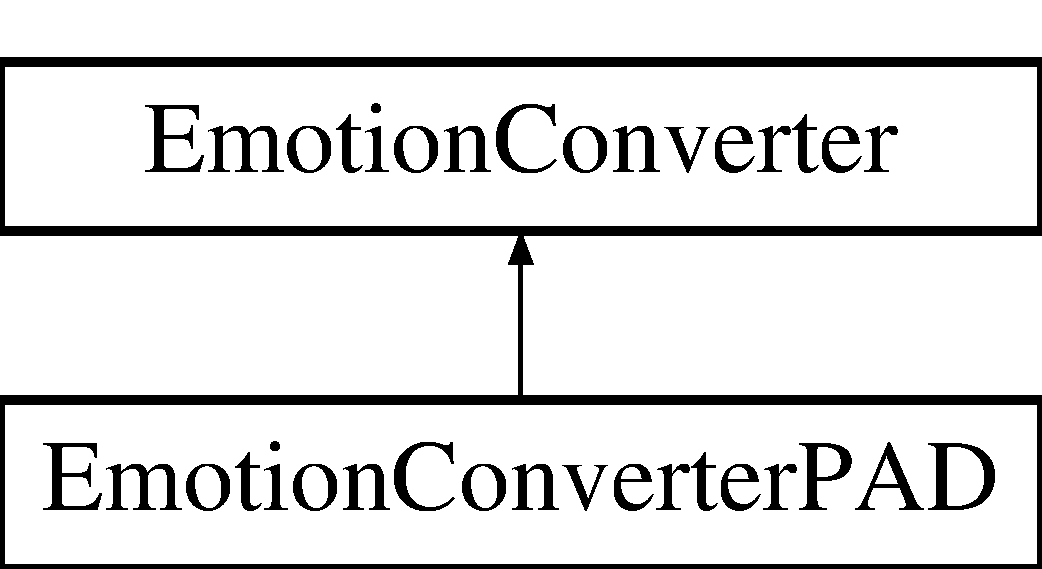
\includegraphics[height=2.000000cm]{class_emotion_converter_p_a_d}
\end{center}
\end{figure}
\subsection*{\-Public \-Member \-Functions}
\begin{DoxyCompactItemize}
\item 
\hyperlink{class_emotion_converter_p_a_d_a672f33449ce967e0f320e8a23b1a9483}{\-Emotion\-Converter\-P\-A\-D} ()
\item 
\hyperlink{class_emotion_converter_p_a_d_a7cd032a614fe93f04323424c70a5ceeb}{$\sim$\-Emotion\-Converter\-P\-A\-D} ()
\item 
std\-::vector$<$ int $>$ \hyperlink{class_emotion_converter_p_a_d_a0bea4550a37916737a01e57255721713}{convert\-To\-Class\-Type} (std\-::vector$<$ int $>$ foreign\-Data)
\item 
std\-::vector$<$ float $>$ \hyperlink{class_emotion_converter_p_a_d_ac1e57bfbadcefdaed62f4a8153709c64}{convert\-From\-Class\-Type} (std\-::vector$<$ float $>$ \-P\-A\-D\-Data)
\item 
\hypertarget{class_emotion_converter_p_a_d_a1ada22855bef77efa0f144b301168967}{
std\-::string {\bfseries to\-String} (std\-::vector$<$ int $>$ \-P\-A\-D\-Data)}
\label{class_emotion_converter_p_a_d_a1ada22855bef77efa0f144b301168967}

\end{DoxyCompactItemize}


\subsection{\-Detailed \-Description}
\-Abbildung vom \-Dynamik-\/\-Raum in den \-P\-A\-D-\/\-Raum nach \-Mehrabian 

\-Definition at line 57 of file \-Emotion\-Converter.\-h.



\subsection{\-Constructor \& \-Destructor \-Documentation}
\hypertarget{class_emotion_converter_p_a_d_a672f33449ce967e0f320e8a23b1a9483}{
\index{\-Emotion\-Converter\-P\-A\-D@{\-Emotion\-Converter\-P\-A\-D}!\-Emotion\-Converter\-P\-A\-D@{\-Emotion\-Converter\-P\-A\-D}}
\index{\-Emotion\-Converter\-P\-A\-D@{\-Emotion\-Converter\-P\-A\-D}!EmotionConverterPAD@{\-Emotion\-Converter\-P\-A\-D}}
\subsubsection[{\-Emotion\-Converter\-P\-A\-D}]{\setlength{\rightskip}{0pt plus 5cm}\-Emotion\-Converter\-P\-A\-D\-::\-Emotion\-Converter\-P\-A\-D (
\begin{DoxyParamCaption}
{}
\end{DoxyParamCaption}
)}}
\label{class_emotion_converter_p_a_d_a672f33449ce967e0f320e8a23b1a9483}
\-Initialisierung der string\-Convert\-Map 

\-Definition at line 48 of file \-Emotion\-Converter.\-cc.

\hypertarget{class_emotion_converter_p_a_d_a7cd032a614fe93f04323424c70a5ceeb}{
\index{\-Emotion\-Converter\-P\-A\-D@{\-Emotion\-Converter\-P\-A\-D}!$\sim$\-Emotion\-Converter\-P\-A\-D@{$\sim$\-Emotion\-Converter\-P\-A\-D}}
\index{$\sim$\-Emotion\-Converter\-P\-A\-D@{$\sim$\-Emotion\-Converter\-P\-A\-D}!EmotionConverterPAD@{\-Emotion\-Converter\-P\-A\-D}}
\subsubsection[{$\sim$\-Emotion\-Converter\-P\-A\-D}]{\setlength{\rightskip}{0pt plus 5cm}\-Emotion\-Converter\-P\-A\-D\-::$\sim$\-Emotion\-Converter\-P\-A\-D (
\begin{DoxyParamCaption}
{}
\end{DoxyParamCaption}
)}}
\label{class_emotion_converter_p_a_d_a7cd032a614fe93f04323424c70a5ceeb}
\-Leerer \-Destruktor. 

\-Definition at line 57 of file \-Emotion\-Converter.\-cc.



\subsection{\-Member \-Function \-Documentation}
\hypertarget{class_emotion_converter_p_a_d_ac1e57bfbadcefdaed62f4a8153709c64}{
\index{\-Emotion\-Converter\-P\-A\-D@{\-Emotion\-Converter\-P\-A\-D}!convert\-From\-Class\-Type@{convert\-From\-Class\-Type}}
\index{convert\-From\-Class\-Type@{convert\-From\-Class\-Type}!EmotionConverterPAD@{\-Emotion\-Converter\-P\-A\-D}}
\subsubsection[{convert\-From\-Class\-Type}]{\setlength{\rightskip}{0pt plus 5cm}std\-::vector$<$ float $>$ \-Emotion\-Converter\-P\-A\-D\-::convert\-From\-Class\-Type (
\begin{DoxyParamCaption}
\item[{std\-::vector$<$ float $>$}]{\-P\-A\-D\-Data}
\end{DoxyParamCaption}
)\hspace{0.3cm}{\ttfamily  \mbox{[}virtual\mbox{]}}}}
\label{class_emotion_converter_p_a_d_ac1e57bfbadcefdaed62f4a8153709c64}
\-We try our best here. 

\-Implements \hyperlink{class_emotion_converter}{\-Emotion\-Converter}.



\-Definition at line 117 of file \-Emotion\-Converter.\-cc.

\hypertarget{class_emotion_converter_p_a_d_a0bea4550a37916737a01e57255721713}{
\index{\-Emotion\-Converter\-P\-A\-D@{\-Emotion\-Converter\-P\-A\-D}!convert\-To\-Class\-Type@{convert\-To\-Class\-Type}}
\index{convert\-To\-Class\-Type@{convert\-To\-Class\-Type}!EmotionConverterPAD@{\-Emotion\-Converter\-P\-A\-D}}
\subsubsection[{convert\-To\-Class\-Type}]{\setlength{\rightskip}{0pt plus 5cm}std\-::vector$<$ int $>$ \-Emotion\-Converter\-P\-A\-D\-::convert\-To\-Class\-Type (
\begin{DoxyParamCaption}
\item[{std\-::vector$<$ int $>$}]{foreign\-Data}
\end{DoxyParamCaption}
)\hspace{0.3cm}{\ttfamily  \mbox{[}virtual\mbox{]}}}}
\label{class_emotion_converter_p_a_d_a0bea4550a37916737a01e57255721713}
\-Hier wird die \-Abbildung \-K(xt, yt, zt, t), wie in der \-Diploamarbeit beschrieben, vorgenommen.

\-Hier wird die \-Abbildung \-K(xt, yt, zt, t), wie in der \-Diploamarbeit beschrieben, vorgenommen. \-N\-E\-W\-: \-Integer values are sufficient! 

\-Implements \hyperlink{class_emotion_converter}{\-Emotion\-Converter}.



\-Definition at line 90 of file \-Emotion\-Converter.\-cc.



\-The documentation for this class was generated from the following files\-:\begin{DoxyCompactItemize}
\item 
\-Emotion\-Converter.\-h\item 
\-Emotion\-Converter.\-cc\end{DoxyCompactItemize}

\hypertarget{class_emotion_dynamics}{
\section{\-Emotion\-Dynamics \-Class \-Reference}
\label{class_emotion_dynamics}\index{\-Emotion\-Dynamics@{\-Emotion\-Dynamics}}
}


{\ttfamily \#include $<$\-Emotion\-Dynamics.\-h$>$}

\-Inheritance diagram for \-Emotion\-Dynamics\-:\begin{figure}[H]
\begin{center}
\leavevmode
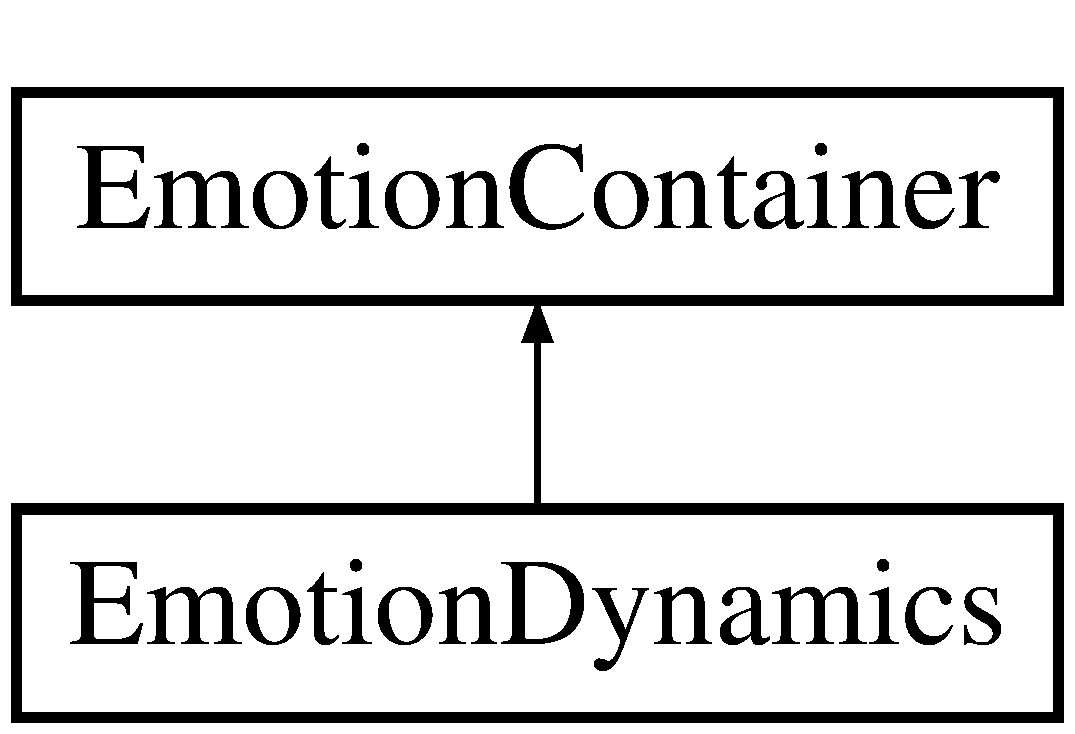
\includegraphics[height=2.000000cm]{class_emotion_dynamics}
\end{center}
\end{figure}
\subsection*{\-Public \-Member \-Functions}
\begin{DoxyCompactItemize}
\item 
\hyperlink{class_emotion_dynamics_a68538ace62b52fcde2d6bc82279dff2d}{$\sim$\-Emotion\-Dynamics} ()
\item 
\hyperlink{class_emotion_dynamics_a836a77ceb1e0590ec148e6739613e960}{\-Emotion\-Dynamics} (const \hyperlink{class_emotion_dynamics}{\-Emotion\-Dynamics} \&emo\-Con)
\item 
virtual void \hyperlink{class_emotion_dynamics_a806fec22c1590ea3df5037bf3922a7b6}{update} (float dt)
\item 
void \hyperlink{class_emotion_dynamics_afd7e47e31ed473b8f16eca21dab04ded}{update} ()
\item 
\hypertarget{class_emotion_dynamics_a156b80db18d99fac37a07b3602c78d46}{
virtual void {\bfseries init} ()}
\label{class_emotion_dynamics_a156b80db18d99fac37a07b3602c78d46}

\item 
\hypertarget{class_emotion_dynamics_a1b034a59d826ef20bac239557b836714}{
bool {\bfseries init\-Emo\-Dyn} ()}
\label{class_emotion_dynamics_a1b034a59d826ef20bac239557b836714}

\item 
\hypertarget{class_emotion_dynamics_a8b3b6aff43f434945d91b38d1ba24c05}{
bool {\bfseries init\-Emo\-P\-A\-D} ()}
\label{class_emotion_dynamics_a8b3b6aff43f434945d91b38d1ba24c05}

\item 
\hypertarget{class_emotion_dynamics_a862799db63e63af7b97f0a8095fecea9}{
virtual void {\bfseries write\-Transferable} (std\-::ostream \&ostr) const }
\label{class_emotion_dynamics_a862799db63e63af7b97f0a8095fecea9}

\item 
\hypertarget{class_emotion_dynamics_ab5a71869fe76988e63567d8da1ebbb0d}{
virtual void {\bfseries read\-Transferable} (std\-::istream \&)}
\label{class_emotion_dynamics_ab5a71869fe76988e63567d8da1ebbb0d}

\end{DoxyCompactItemize}
\subsection*{\-Public \-Attributes}
\begin{DoxyCompactItemize}
\item 
\hypertarget{class_emotion_dynamics_a785aa6925251548729a83d13cf33cfaa}{
std\-::string {\bfseries dyn\-Filename}}
\label{class_emotion_dynamics_a785aa6925251548729a83d13cf33cfaa}

\item 
\hypertarget{class_emotion_dynamics_a609f12ad220dd954278e9c229caff863}{
std\-::string {\bfseries pad\-Filename}}
\label{class_emotion_dynamics_a609f12ad220dd954278e9c229caff863}

\item 
\hypertarget{class_emotion_dynamics_a468bde5060ab501eac7766f8c8af237b}{
int {\bfseries spon\-\_\-target}}
\label{class_emotion_dynamics_a468bde5060ab501eac7766f8c8af237b}

\item 
\hypertarget{class_emotion_dynamics_a6f437f85dbb70ef001042290adeb2bcc}{
int {\bfseries prev\-\_\-target}}
\label{class_emotion_dynamics_a6f437f85dbb70ef001042290adeb2bcc}

\item 
\hypertarget{class_emotion_dynamics_a137fb40b93d6fbc83306ba46f1e86bb5}{
int {\bfseries dom\-\_\-target}}
\label{class_emotion_dynamics_a137fb40b93d6fbc83306ba46f1e86bb5}

\item 
\hypertarget{class_emotion_dynamics_a8022ce5df1dee1d1c82f2118620c5e77}{
double {\bfseries mass}}
\label{class_emotion_dynamics_a8022ce5df1dee1d1c82f2118620c5e77}

\item 
\hypertarget{class_emotion_dynamics_a3cde6fcb41a079c1ec589a864b1756da}{
double {\bfseries sxlast}}
\label{class_emotion_dynamics_a3cde6fcb41a079c1ec589a864b1756da}

\item 
\hypertarget{class_emotion_dynamics_a178bc78f21560e73099f442b110ac72a}{
double {\bfseries sylast}}
\label{class_emotion_dynamics_a178bc78f21560e73099f442b110ac72a}

\item 
\hypertarget{class_emotion_dynamics_ab343e535c5040bd196d16d7a7208466f}{
double {\bfseries sxt}}
\label{class_emotion_dynamics_ab343e535c5040bd196d16d7a7208466f}

\item 
\hypertarget{class_emotion_dynamics_ae5e489a52ca972a89cfcef3f7560eecd}{
double {\bfseries syt}}
\label{class_emotion_dynamics_ae5e489a52ca972a89cfcef3f7560eecd}

\item 
\hypertarget{class_emotion_dynamics_a3f83131653bbcb3cc7d33e275d0e68fc}{
double {\bfseries sdom}}
\label{class_emotion_dynamics_a3f83131653bbcb3cc7d33e275d0e68fc}

\item 
\hypertarget{class_emotion_dynamics_afcf2988c58857bf4097203862fea7147}{
double {\bfseries sdomlast}}
\label{class_emotion_dynamics_afcf2988c58857bf4097203862fea7147}

\item 
\hypertarget{class_emotion_dynamics_aa105dfb370d4d61c9f5d1541585ddde0}{
double {\bfseries vxlast}}
\label{class_emotion_dynamics_aa105dfb370d4d61c9f5d1541585ddde0}

\item 
\hypertarget{class_emotion_dynamics_a91be7910f8de0b8d547fcd9108b0efdc}{
double {\bfseries vylast}}
\label{class_emotion_dynamics_a91be7910f8de0b8d547fcd9108b0efdc}

\item 
\hypertarget{class_emotion_dynamics_aad3f84224f9ed8090c685726b998fd72}{
double {\bfseries vxt}}
\label{class_emotion_dynamics_aad3f84224f9ed8090c685726b998fd72}

\item 
\hypertarget{class_emotion_dynamics_ab79fa9eb9528136f6f8e1841efb44f75}{
double {\bfseries vyt}}
\label{class_emotion_dynamics_ab79fa9eb9528136f6f8e1841efb44f75}

\item 
\hypertarget{class_emotion_dynamics_a0291d5b3750e65b8f3c2fae1d496aaaf}{
double {\bfseries vdom}}
\label{class_emotion_dynamics_a0291d5b3750e65b8f3c2fae1d496aaaf}

\item 
\hypertarget{class_emotion_dynamics_a7422bc00f622ff8a8ee2d4540660bda7}{
double {\bfseries vdomlast}}
\label{class_emotion_dynamics_a7422bc00f622ff8a8ee2d4540660bda7}

\item 
\hypertarget{class_emotion_dynamics_a50315c4ed074e5aa05602b407b567a90}{
double {\bfseries axlast}}
\label{class_emotion_dynamics_a50315c4ed074e5aa05602b407b567a90}

\item 
\hypertarget{class_emotion_dynamics_af0ce936165f587e37425cc482efc33fd}{
double {\bfseries aylast}}
\label{class_emotion_dynamics_af0ce936165f587e37425cc482efc33fd}

\item 
\hypertarget{class_emotion_dynamics_a4914dbeaca6882719942ba95a3d4fdb7}{
double {\bfseries axt}}
\label{class_emotion_dynamics_a4914dbeaca6882719942ba95a3d4fdb7}

\item 
\hypertarget{class_emotion_dynamics_a29f2a61cfd95c3395e811980b00d36d1}{
double {\bfseries ayt}}
\label{class_emotion_dynamics_a29f2a61cfd95c3395e811980b00d36d1}

\item 
\hypertarget{class_emotion_dynamics_a362ca6d7dc604be1d7dd8d09f7e3f61b}{
double {\bfseries adom}}
\label{class_emotion_dynamics_a362ca6d7dc604be1d7dd8d09f7e3f61b}

\item 
\hypertarget{class_emotion_dynamics_a7b8378fd5de2cd38498f0e0ed0d1f4bb}{
double {\bfseries adomlast}}
\label{class_emotion_dynamics_a7b8378fd5de2cd38498f0e0ed0d1f4bb}

\item 
\hypertarget{class_emotion_dynamics_ab3ad74329483a05c82f5dd837e5761fe}{
double {\bfseries z}}
\label{class_emotion_dynamics_ab3ad74329483a05c82f5dd837e5761fe}

\item 
\hypertarget{class_emotion_dynamics_a315aebaa8e927183734cec16966af8cb}{
bool {\bfseries x\-Sign\-Change}}
\label{class_emotion_dynamics_a315aebaa8e927183734cec16966af8cb}

\item 
\hypertarget{class_emotion_dynamics_a9ef0cad8e968f60c000a287b57dc85b5}{
bool {\bfseries y\-Sign\-Change}}
\label{class_emotion_dynamics_a9ef0cad8e968f60c000a287b57dc85b5}

\item 
\hypertarget{class_emotion_dynamics_a58e6db5700a9d3fd0c616e12e2a4a0d1}{
int {\bfseries x\-Sign}}
\label{class_emotion_dynamics_a58e6db5700a9d3fd0c616e12e2a4a0d1}

\item 
\hypertarget{class_emotion_dynamics_a6730f7847ceda83a39164e1d75c49906}{
int {\bfseries y\-Sign}}
\label{class_emotion_dynamics_a6730f7847ceda83a39164e1d75c49906}

\item 
\hypertarget{class_emotion_dynamics_a9b5768aa0f49fa87ca6885634ffa73c3}{
\hyperlink{class_emo_pos2_reach}{\-Emo\-Pos2\-Reach} $\ast$ {\bfseries positions2\-Reach}}
\label{class_emotion_dynamics_a9b5768aa0f49fa87ca6885634ffa73c3}

\item 
\hypertarget{class_emotion_dynamics_a775cf992332ff49c0fb8cabd1643fe5b}{
int {\bfseries x\-Tens}}
\label{class_emotion_dynamics_a775cf992332ff49c0fb8cabd1643fe5b}

\item 
\hypertarget{class_emotion_dynamics_ac432577cfd7bb4b3e556ade2a5ac435a}{
int {\bfseries y\-Tens}}
\label{class_emotion_dynamics_ac432577cfd7bb4b3e556ade2a5ac435a}

\item 
\hypertarget{class_emotion_dynamics_af9577f55643cc20ea444803bd282aa1e}{
int {\bfseries slope}}
\label{class_emotion_dynamics_af9577f55643cc20ea444803bd282aa1e}

\item 
\hypertarget{class_emotion_dynamics_ae49c90d9fdf4eba4854773c0acc382d0}{
int {\bfseries x\-Reg}}
\label{class_emotion_dynamics_ae49c90d9fdf4eba4854773c0acc382d0}

\item 
\hypertarget{class_emotion_dynamics_ad283e4f8cc06edb85cf2a43f29a006fc}{
int {\bfseries y\-Reg}}
\label{class_emotion_dynamics_ad283e4f8cc06edb85cf2a43f29a006fc}

\item 
\hypertarget{class_emotion_dynamics_ad6b40429659516e168aa33ebb6c116b1}{
int {\bfseries boredom}}
\label{class_emotion_dynamics_ad6b40429659516e168aa33ebb6c116b1}

\item 
\hypertarget{class_emotion_dynamics_accb6a1b571b75ed144754c38165dc102}{
int {\bfseries mean}}
\label{class_emotion_dynamics_accb6a1b571b75ed144754c38165dc102}

\item 
\hypertarget{class_emotion_dynamics_a4454cece93b0e0d32dfbced9a0490926}{
float {\bfseries last\-Update}}
\label{class_emotion_dynamics_a4454cece93b0e0d32dfbced9a0490926}

\item 
\hypertarget{class_emotion_dynamics_a55320fb65b8174096af3415d093fc6f9}{
int {\bfseries x\-Pos}}
\label{class_emotion_dynamics_a55320fb65b8174096af3415d093fc6f9}

\item 
\hypertarget{class_emotion_dynamics_adabc8203c0a55205eaed8722816e993a}{
int {\bfseries y\-Pos}}
\label{class_emotion_dynamics_adabc8203c0a55205eaed8722816e993a}

\item 
\hypertarget{class_emotion_dynamics_a555a8bb2c434a2245e5d7cae575aa9bb}{
int {\bfseries z\-Pos}}
\label{class_emotion_dynamics_a555a8bb2c434a2245e5d7cae575aa9bb}

\item 
\hypertarget{class_emotion_dynamics_a4e5c5b303ec5bff429fcaa9b8f9ac9c5}{
int {\bfseries p\-Value}}
\label{class_emotion_dynamics_a4e5c5b303ec5bff429fcaa9b8f9ac9c5}

\item 
\hypertarget{class_emotion_dynamics_a52a013b50284ba08c12d30ccc9b35b5d}{
int {\bfseries a\-Value}}
\label{class_emotion_dynamics_a52a013b50284ba08c12d30ccc9b35b5d}

\item 
\hypertarget{class_emotion_dynamics_ad12dad0868568048b1fb973210dbaa58}{
int {\bfseries d\-Value}}
\label{class_emotion_dynamics_ad12dad0868568048b1fb973210dbaa58}

\end{DoxyCompactItemize}


\subsection{\-Detailed \-Description}
\-This class implements the emotion dynamics. \-It is derived from \hyperlink{class_emotion_container}{\-Emotion\-Container} and reimplements the update-\/function 

\-Definition at line 37 of file \-Emotion\-Dynamics.\-h.



\subsection{\-Constructor \& \-Destructor \-Documentation}
\hypertarget{class_emotion_dynamics_a68538ace62b52fcde2d6bc82279dff2d}{
\index{\-Emotion\-Dynamics@{\-Emotion\-Dynamics}!$\sim$\-Emotion\-Dynamics@{$\sim$\-Emotion\-Dynamics}}
\index{$\sim$\-Emotion\-Dynamics@{$\sim$\-Emotion\-Dynamics}!EmotionDynamics@{\-Emotion\-Dynamics}}
\subsubsection[{$\sim$\-Emotion\-Dynamics}]{\setlength{\rightskip}{0pt plus 5cm}\-Emotion\-Dynamics\-::$\sim$\-Emotion\-Dynamics (
\begin{DoxyParamCaption}
{}
\end{DoxyParamCaption}
)}}
\label{class_emotion_dynamics_a68538ace62b52fcde2d6bc82279dff2d}
\-Deleting positions2\-Reach 

\-Definition at line 66 of file \-Emotion\-Dynamics.\-cc.

\hypertarget{class_emotion_dynamics_a836a77ceb1e0590ec148e6739613e960}{
\index{\-Emotion\-Dynamics@{\-Emotion\-Dynamics}!\-Emotion\-Dynamics@{\-Emotion\-Dynamics}}
\index{\-Emotion\-Dynamics@{\-Emotion\-Dynamics}!EmotionDynamics@{\-Emotion\-Dynamics}}
\subsubsection[{\-Emotion\-Dynamics}]{\setlength{\rightskip}{0pt plus 5cm}\-Emotion\-Dynamics\-::\-Emotion\-Dynamics (
\begin{DoxyParamCaption}
\item[{const {\bf \-Emotion\-Dynamics} \&}]{emo\-Con}
\end{DoxyParamCaption}
)}}
\label{class_emotion_dynamics_a836a77ceb1e0590ec148e6739613e960}
\-Simple \-Copy \-Constructor 

\-Definition at line 75 of file \-Emotion\-Dynamics.\-cc.



\subsection{\-Member \-Function \-Documentation}
\hypertarget{class_emotion_dynamics_a806fec22c1590ea3df5037bf3922a7b6}{
\index{\-Emotion\-Dynamics@{\-Emotion\-Dynamics}!update@{update}}
\index{update@{update}!EmotionDynamics@{\-Emotion\-Dynamics}}
\subsubsection[{update}]{\setlength{\rightskip}{0pt plus 5cm}void \-Emotion\-Dynamics\-::update (
\begin{DoxyParamCaption}
\item[{float}]{\-\_\-dt}
\end{DoxyParamCaption}
)\hspace{0.3cm}{\ttfamily  \mbox{[}virtual\mbox{]}}}}
\label{class_emotion_dynamics_a806fec22c1590ea3df5037bf3922a7b6}
\-Physics calculation for x-\/value (emotion) as described in \-Ph\-D thesis.

\-In addition, the y-\/value (mood) is calculated as follows\-: \-By means of \hyperlink{class_emo_pos2_reach}{\-Emo\-Pos2\-Reach} contained in \hyperlink{class_emotion_container}{\-Emotion\-Container}, of which this class is a subclass, an integer y\-Pos2\-Reach is being managed as well as a boolean, which can be checked using \-Emo\-Pos2\-Reach-\/$>$get\-Y\-Valid(). \-If this returns true, the achor point of the spiral spring for y is temporarily attached to the y\-Pos2\-Reach value (indicated by a blue circle in \-P\-A\-D space). \-Consequently, a force is applied to the reference point, by which it is driven towards y\-Pos2\-Reach. \-After reaching it, the forces are reset to zero and y\-Pos2\-Reach-\/$>$set\-Valid(false) executed. \-The y coordinate is, thus, again driven back to 0 over time. 

\-Reimplemented from \hyperlink{class_emotion_container_a8c63f4c9e9c558b4cecdf1aab9c81bd0}{\-Emotion\-Container}.



\-Definition at line 142 of file \-Emotion\-Dynamics.\-cc.

\hypertarget{class_emotion_dynamics_afd7e47e31ed473b8f16eca21dab04ded}{
\index{\-Emotion\-Dynamics@{\-Emotion\-Dynamics}!update@{update}}
\index{update@{update}!EmotionDynamics@{\-Emotion\-Dynamics}}
\subsubsection[{update}]{\setlength{\rightskip}{0pt plus 5cm}void \-Emotion\-Dynamics\-::update (
\begin{DoxyParamCaption}
{}
\end{DoxyParamCaption}
)}}
\label{class_emotion_dynamics_afd7e47e31ed473b8f16eca21dab04ded}
\-If we dont get a dt value, we use our internal dt 

\-Definition at line 123 of file \-Emotion\-Dynamics.\-cc.



\-The documentation for this class was generated from the following files\-:\begin{DoxyCompactItemize}
\item 
\-Emotion\-Dynamics.\-h\item 
\-Emotion\-Dynamics.\-cc\end{DoxyCompactItemize}

\hypertarget{class_primary_emotion}{
\section{\-Primary\-Emotion \-Class \-Reference}
\label{class_primary_emotion}\index{\-Primary\-Emotion@{\-Primary\-Emotion}}
}
\-Inheritance diagram for \-Primary\-Emotion\-:\begin{figure}[H]
\begin{center}
\leavevmode
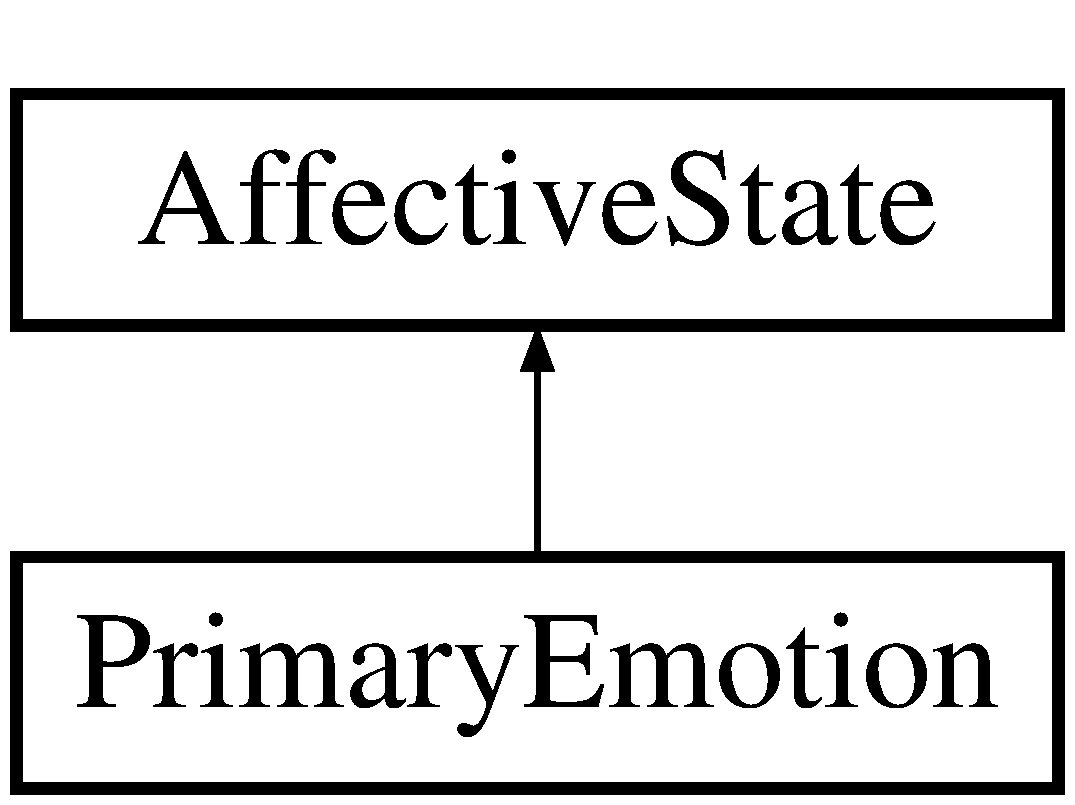
\includegraphics[height=2.000000cm]{class_primary_emotion}
\end{center}
\end{figure}
\subsection*{\-Public \-Member \-Functions}
\begin{DoxyCompactItemize}
\item 
\hypertarget{class_primary_emotion_a1e27423637ba33eb1a1c8910cab29608}{
{\bfseries \-Primary\-Emotion} (std\-::vector$<$ \hyperlink{class_affect_polygon}{\-Affect\-Polygon} $\ast$ $>$ ap\-\_\-vec)}
\label{class_primary_emotion_a1e27423637ba33eb1a1c8910cab29608}

\item 
\hypertarget{class_primary_emotion_af804796c1d91c359a8ae1d4173a05011}{
{\bfseries \-Primary\-Emotion} (\hyperlink{class_affect_polygon}{\-Affect\-Polygon} $\ast$ap)}
\label{class_primary_emotion_af804796c1d91c359a8ae1d4173a05011}

\item 
\hypertarget{class_primary_emotion_a930ff9585427165598b3624c7732eb15}{
bool {\bfseries add\-To\-Secondary\-Emotion} (\hyperlink{class_secondary_emotion}{\-Secondary\-Emotion} $\ast$se)}
\label{class_primary_emotion_a930ff9585427165598b3624c7732eb15}

\end{DoxyCompactItemize}
\subsection*{\-Protected \-Attributes}
\begin{DoxyCompactItemize}
\item 
\hypertarget{class_primary_emotion_aa56575b1b520f26199ce41ce466218cd}{
std\-::vector$<$ \hyperlink{class_secondary_emotion}{\-Secondary\-Emotion} $\ast$ $>$ {\bfseries used\-By\-Secondary\-Emotions}}
\label{class_primary_emotion_aa56575b1b520f26199ce41ce466218cd}

\end{DoxyCompactItemize}


\subsection{\-Detailed \-Description}


\-Definition at line 38 of file \-Primary\-Emotion.\-h.



\-The documentation for this class was generated from the following files\-:\begin{DoxyCompactItemize}
\item 
\-Primary\-Emotion.\-h\item 
\-Affective\-State.\-cc\item 
\-Primary\-Emotion.\-cc\end{DoxyCompactItemize}

\hypertarget{class_secondary_emotion}{
\section{\-Secondary\-Emotion \-Class \-Reference}
\label{class_secondary_emotion}\index{\-Secondary\-Emotion@{\-Secondary\-Emotion}}
}
\-Inheritance diagram for \-Secondary\-Emotion\-:\begin{figure}[H]
\begin{center}
\leavevmode
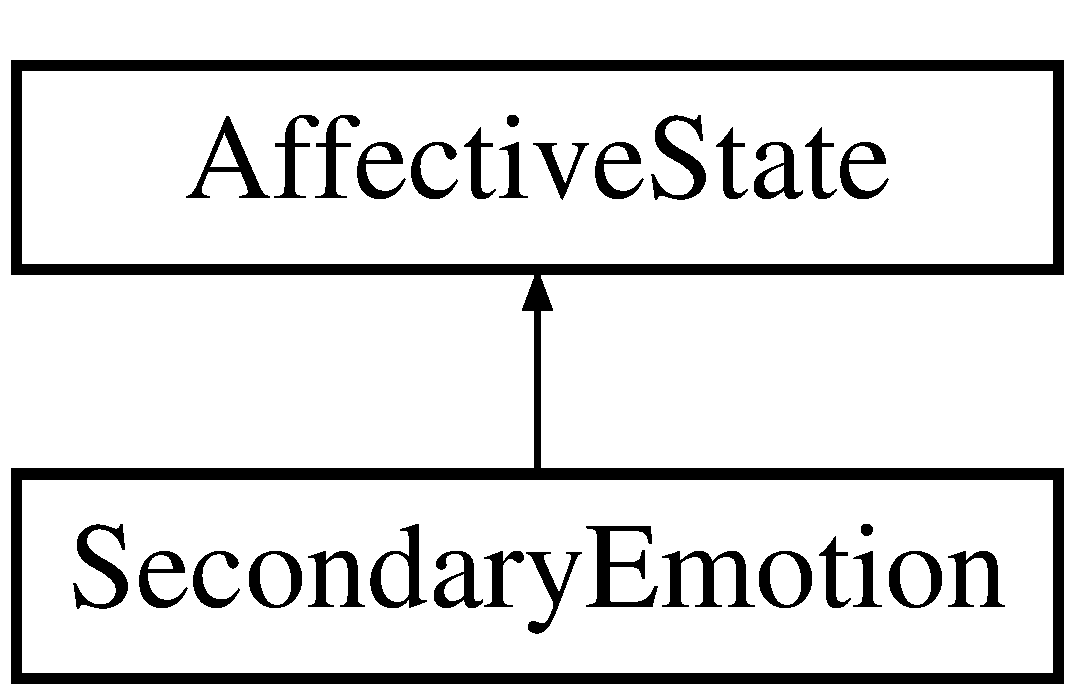
\includegraphics[height=2.000000cm]{class_secondary_emotion}
\end{center}
\end{figure}
\subsection*{\-Public \-Member \-Functions}
\begin{DoxyCompactItemize}
\item 
\hypertarget{class_secondary_emotion_a28d618dbf5942bede4212aa865ad5584}{
{\bfseries \-Secondary\-Emotion} (std\-::vector$<$ \hyperlink{class_affect_polygon}{\-Affect\-Polygon} $\ast$ $>$ ap\-\_\-vec)}
\label{class_secondary_emotion_a28d618dbf5942bede4212aa865ad5584}

\item 
\hypertarget{class_secondary_emotion_afccda0194ecd624c80431086edbf585d}{
{\bfseries \-Secondary\-Emotion} (\hyperlink{class_affect_polygon}{\-Affect\-Polygon} $\ast$ap)}
\label{class_secondary_emotion_afccda0194ecd624c80431086edbf585d}

\item 
\hypertarget{class_secondary_emotion_ae66a9c880c5b443ff0c8ca2157811ea9}{
bool {\bfseries load\-From\-File} (std\-::string filename)}
\label{class_secondary_emotion_ae66a9c880c5b443ff0c8ca2157811ea9}

\item 
\hypertarget{class_secondary_emotion_a048337e8bf8c3a8ccc8caf68ac7d4783}{
void {\bfseries add\-Primary\-Emotion} (\hyperlink{class_primary_emotion}{\-Primary\-Emotion} $\ast$pe)}
\label{class_secondary_emotion_a048337e8bf8c3a8ccc8caf68ac7d4783}

\end{DoxyCompactItemize}
\subsection*{\-Protected \-Attributes}
\begin{DoxyCompactItemize}
\item 
\hypertarget{class_secondary_emotion_a9715b0f8a820b8d190ce097c31750388}{
std\-::vector$<$ \hyperlink{class_primary_emotion}{\-Primary\-Emotion} $\ast$ $>$ {\bfseries uses\-Primary\-Emotions}}
\label{class_secondary_emotion_a9715b0f8a820b8d190ce097c31750388}

\end{DoxyCompactItemize}


\subsection{\-Detailed \-Description}


\-Definition at line 37 of file \-Secondary\-Emotion.\-h.



\-The documentation for this class was generated from the following files\-:\begin{DoxyCompactItemize}
\item 
\-Secondary\-Emotion.\-h\item 
\-Secondary\-Emotion.\-cc\end{DoxyCompactItemize}

\hypertarget{class_w_a_s_a_b_i_engine}{
\section{\-W\-A\-S\-A\-B\-I\-Engine \-Class \-Reference}
\label{class_w_a_s_a_b_i_engine}\index{\-W\-A\-S\-A\-B\-I\-Engine@{\-W\-A\-S\-A\-B\-I\-Engine}}
}
\subsection*{\-Public \-Member \-Functions}
\begin{DoxyCompactItemize}
\item 
\hypertarget{class_w_a_s_a_b_i_engine_a540e648058255c16b40d44307fb5b3d4}{
{\bfseries \-W\-A\-S\-A\-B\-I\-Engine} (std\-::string emotionclass=\char`\"{}primary\char`\"{})}
\label{class_w_a_s_a_b_i_engine_a540e648058255c16b40d44307fb5b3d4}

\item 
\hypertarget{class_w_a_s_a_b_i_engine_a1f423672efd6835807341801d6acc5c9}{
void {\bfseries init\-Class} ()}
\label{class_w_a_s_a_b_i_engine_a1f423672efd6835807341801d6acc5c9}

\item 
\hypertarget{class_w_a_s_a_b_i_engine_a3bff7681c6bb49d1b6bfd3aa351c2d22}{
\hyperlink{classcoga_emotional_attendee}{coga\-Emotional\-Attendee} $\ast$ {\bfseries get\-E\-Afrom\-I\-D} (int uid=1)}
\label{class_w_a_s_a_b_i_engine_a3bff7681c6bb49d1b6bfd3aa351c2d22}

\item 
\hypertarget{class_w_a_s_a_b_i_engine_a04703a0f51c836c5289ae40311bfda5d}{
\hyperlink{classcoga_emotional_attendee}{coga\-Emotional\-Attendee} $\ast$ {\bfseries get\-E\-Afrom\-I\-D} (std\-::string global\-I\-D)}
\label{class_w_a_s_a_b_i_engine_a04703a0f51c836c5289ae40311bfda5d}

\item 
\hypertarget{class_w_a_s_a_b_i_engine_a1ca90c61e77cc5c2495ed877f19c9872}{
void {\bfseries init\-All\-E\-As} ()}
\label{class_w_a_s_a_b_i_engine_a1ca90c61e77cc5c2495ed877f19c9872}

\item 
\hypertarget{class_w_a_s_a_b_i_engine_a8c2418e79b911f27069db8bcc8678385}{
bool {\bfseries init\-E\-A} (\hyperlink{classcoga_emotional_attendee}{coga\-Emotional\-Attendee} $\ast$ea)}
\label{class_w_a_s_a_b_i_engine_a8c2418e79b911f27069db8bcc8678385}

\item 
\hypertarget{class_w_a_s_a_b_i_engine_aec2bc2264141f0e458c04c80806c5bc4}{
bool {\bfseries update} ()}
\label{class_w_a_s_a_b_i_engine_aec2bc2264141f0e458c04c80806c5bc4}

\item 
bool \hyperlink{class_w_a_s_a_b_i_engine_ab36d4f1e86abe80bc29a636641995d74}{get\-P\-A\-D\-String} (std\-::string \&pad\-String, int uid=1)
\item 
\hypertarget{class_w_a_s_a_b_i_engine_aa1f6c88567e14b2f8e18c20682d95555}{
bool {\bfseries emotional\-Impulse} (int impulse, int uid=1)}
\label{class_w_a_s_a_b_i_engine_aa1f6c88567e14b2f8e18c20682d95555}

\item 
\hypertarget{class_w_a_s_a_b_i_engine_aad56212e9e16d3aca7c93184e22ea527}{
bool {\bfseries reset\-To\-Zero} (int uid=1)}
\label{class_w_a_s_a_b_i_engine_aad56212e9e16d3aca7c93184e22ea527}

\item 
\hypertarget{class_w_a_s_a_b_i_engine_a6ef66887c993bd63b413186e8164830b}{
bool {\bfseries set\-X\-Force} (int value, int uid=1)}
\label{class_w_a_s_a_b_i_engine_a6ef66887c993bd63b413186e8164830b}

\item 
\hypertarget{class_w_a_s_a_b_i_engine_a65f302732da8469c219752b118861d99}{
bool {\bfseries set\-Y\-Force} (int value, int uid=1)}
\label{class_w_a_s_a_b_i_engine_a65f302732da8469c219752b118861d99}

\item 
\hypertarget{class_w_a_s_a_b_i_engine_ac02ba44929c3f3c3c43a8b192736e39c}{
bool {\bfseries set\-Slope} (int value, int uid=1)}
\label{class_w_a_s_a_b_i_engine_ac02ba44929c3f3c3c43a8b192736e39c}

\item 
\hypertarget{class_w_a_s_a_b_i_engine_aaf3be59b72800f2b6d4e036c12206308}{
bool {\bfseries set\-Mass} (int value, int uid=1)}
\label{class_w_a_s_a_b_i_engine_aaf3be59b72800f2b6d4e036c12206308}

\item 
\hypertarget{class_w_a_s_a_b_i_engine_a21e4b22ca625bb3cb0944be3fe4d57b1}{
bool {\bfseries set\-Update\-Rate} (int value, int uid=1)}
\label{class_w_a_s_a_b_i_engine_a21e4b22ca625bb3cb0944be3fe4d57b1}

\item 
\hypertarget{class_w_a_s_a_b_i_engine_aad9d281c287559ba4efeae7ae1ed3dbb}{
bool {\bfseries set\-Alpha} (int value, int uid=1)}
\label{class_w_a_s_a_b_i_engine_aad9d281c287559ba4efeae7ae1ed3dbb}

\item 
\hypertarget{class_w_a_s_a_b_i_engine_aef5549ff1ae5cebe145a3ab2fd46d598}{
bool {\bfseries set\-Beta} (int value, int uid=1)}
\label{class_w_a_s_a_b_i_engine_aef5549ff1ae5cebe145a3ab2fd46d598}

\item 
\hypertarget{class_w_a_s_a_b_i_engine_a0a4999f62ff8e228469b778585c55831}{
bool {\bfseries set\-Factor} (int value, int uid=1)}
\label{class_w_a_s_a_b_i_engine_a0a4999f62ff8e228469b778585c55831}

\item 
\hypertarget{class_w_a_s_a_b_i_engine_a528d8baced03e67e11439c8a04f9e6a3}{
void {\bfseries set\-Max\-Simulations} (int max)}
\label{class_w_a_s_a_b_i_engine_a528d8baced03e67e11439c8a04f9e6a3}

\item 
\hypertarget{class_w_a_s_a_b_i_engine_a8dbfcd81addce75eb03fe784f8596b2e}{
int {\bfseries add\-Emotional\-Attendee} (std\-::string name, std\-::string global\-I\-D=\char`\"{}undef\char`\"{}, std\-::string init\-Filename=\char`\"{}init\char`\"{})}
\label{class_w_a_s_a_b_i_engine_a8dbfcd81addce75eb03fe784f8596b2e}

\end{DoxyCompactItemize}
\subsection*{\-Public \-Attributes}
\begin{DoxyCompactItemize}
\item 
\hypertarget{class_w_a_s_a_b_i_engine_aec54c4d7d1debc3f77df23d746550291}{
std\-::vector\*
$<$ \hyperlink{classcoga_emotional_attendee}{coga\-Emotional\-Attendee} $\ast$ $>$ {\bfseries emo\-Attendees}}
\label{class_w_a_s_a_b_i_engine_aec54c4d7d1debc3f77df23d746550291}

\item 
\hypertarget{class_w_a_s_a_b_i_engine_aad318caa6298309bab74ca37ea69ce59}{
std\-::string {\bfseries \-Class}}
\label{class_w_a_s_a_b_i_engine_aad318caa6298309bab74ca37ea69ce59}

\end{DoxyCompactItemize}


\subsection{\-Detailed \-Description}


\-Definition at line 32 of file \-W\-A\-S\-A\-B\-I\-Engine.\-h.



\subsection{\-Member \-Function \-Documentation}
\hypertarget{class_w_a_s_a_b_i_engine_ab36d4f1e86abe80bc29a636641995d74}{
\index{\-W\-A\-S\-A\-B\-I\-Engine@{\-W\-A\-S\-A\-B\-I\-Engine}!get\-P\-A\-D\-String@{get\-P\-A\-D\-String}}
\index{get\-P\-A\-D\-String@{get\-P\-A\-D\-String}!WASABIEngine@{\-W\-A\-S\-A\-B\-I\-Engine}}
\subsubsection[{get\-P\-A\-D\-String}]{\setlength{\rightskip}{0pt plus 5cm}bool \-W\-A\-S\-A\-B\-I\-Engine\-::get\-P\-A\-D\-String (
\begin{DoxyParamCaption}
\item[{std\-::string \&}]{pad\-String, }
\item[{int}]{uid = {\ttfamily 1}}
\end{DoxyParamCaption}
)}}
\label{class_w_a_s_a_b_i_engine_ab36d4f1e86abe80bc29a636641995d74}
retrieve the pad\-String for the \hyperlink{classcoga_emotional_attendee}{coga\-Emotional\-Attendee} with matching uid return false in case of failure, fill string pad\-String and return true otherwise 

\-Definition at line 87 of file \-W\-A\-S\-A\-B\-I\-Engine.\-cc.



\-The documentation for this class was generated from the following files\-:\begin{DoxyCompactItemize}
\item 
\-W\-A\-S\-A\-B\-I\-Engine.\-h\item 
\-W\-A\-S\-A\-B\-I\-Engine.\-cc\end{DoxyCompactItemize}

\printindex
\end{document}
